\documentclass[a4paper, openany]{memoir}

\usepackage[utf8]{inputenc}
\usepackage[T1]{fontenc} 
\usepackage[english]{babel}

\usepackage{fancyhdr}
\usepackage{float}

\usepackage{amsmath}
\usepackage{amsthm}
\usepackage{amssymb}
\usepackage{enumitem}
\usepackage{multicol}
\usepackage[bookmarksopen=true,bookmarksopenlevel=2]{hyperref}
\usepackage{tikz}
\usepackage{indentfirst}

\pagestyle{fancy}
\fancyhf{}
\fancyhead[LE]{\leftmark}
\fancyhead[RO]{\rightmark}
\fancyhead[RE, LO]{Data Fundamentals}
\fancyfoot[LE, RO]{\thepage}
\fancyfoot[RE, LO]{Pete Gautam}

\renewcommand{\headrulewidth}{1.5pt}

\chapterstyle{thatcher}
\setcounter{chapter}{1}
\begin{document}

\chapter{Scientific Visualisation}
\section{Introduction to Visualisation}
Visualisation is the presentation of data. It is used to:
\begin{itemize}
    \item build intuition about the patterns within data;
    \item summarise a large amount of data; and
    \item help see patterns/answer a question about the data easily/quickly.
\end{itemize}
In this course, we will look at displaying 3 basic categories of data:
\begin{itemize}
    \item plots of single 1D array, e.g. histograms (one column);
    \item plots of pairs of 1D arrays, e.g. scatterplots (two columns); and
    \item plots of single 2D arrays, e.g. contour plots (whole table).
\end{itemize}

\subsection{Grammar of Graphics}
The following terminologies are used when describing graphics.
\begin{itemize}
    \item stat: A statistic computed from the dataset\sidefootnote{Dataset is a table of numbers.} to allow the data to be summarised compactly in a graphic (e.g. mean, value, standard deviation bars, binning values in a histogram, etc.).
    
    \item mapping: A transformation of data into visual values- maps stats and raw values from the dataset to visual values, with a scale:
    \begin{itemize}
        \item scale: A scale specifies the transformation of units in the dataset/stat to visual units, e.g. meter scale to $x$ position, altitude to colours. It also specifies the range of values to be mapped.
        \item guide: A visual reference that explains the meaning of the mapping, including the scale and the attribute, e.g. axis, tick marks, labels, colour scales, legends, etc.
    \end{itemize}

    \item geom: A geometric representation of the data after it has been mapped, e.g. points (which have attribute shape, size and colour), lines (which have attributes size, dash styles, thickness, etc.) and patches/polygons.
    
    \item coord: A coordinate system, which connects mapped data onto points on the plane/3D position/etc; the layout of the geoms and guides depends on the coordinate system.
    
    \item layer: One set of geoms, with one mapping to the coordinate system. There can be multiple layers on the same coordinate system, e.g. two stats may be plotted on different layers, but the same coordinate system.
    
    \item facet: Different views of the same dataset, on a different coordinate system, e.g. two conditions of an experiment may be plotted on two different facets. One fact can have multiple layers, all plotted on the same coordinate system.
    
    \item figure: A set of one or more facets.
    
    \item caption: A description of the visualisation. A figure must have a caption.
\end{itemize}
\noindent Altogether, this is called the Layered Grammar of Graphics. A pictorial representation is given below:
\begin{figure}[H]
    \centering
    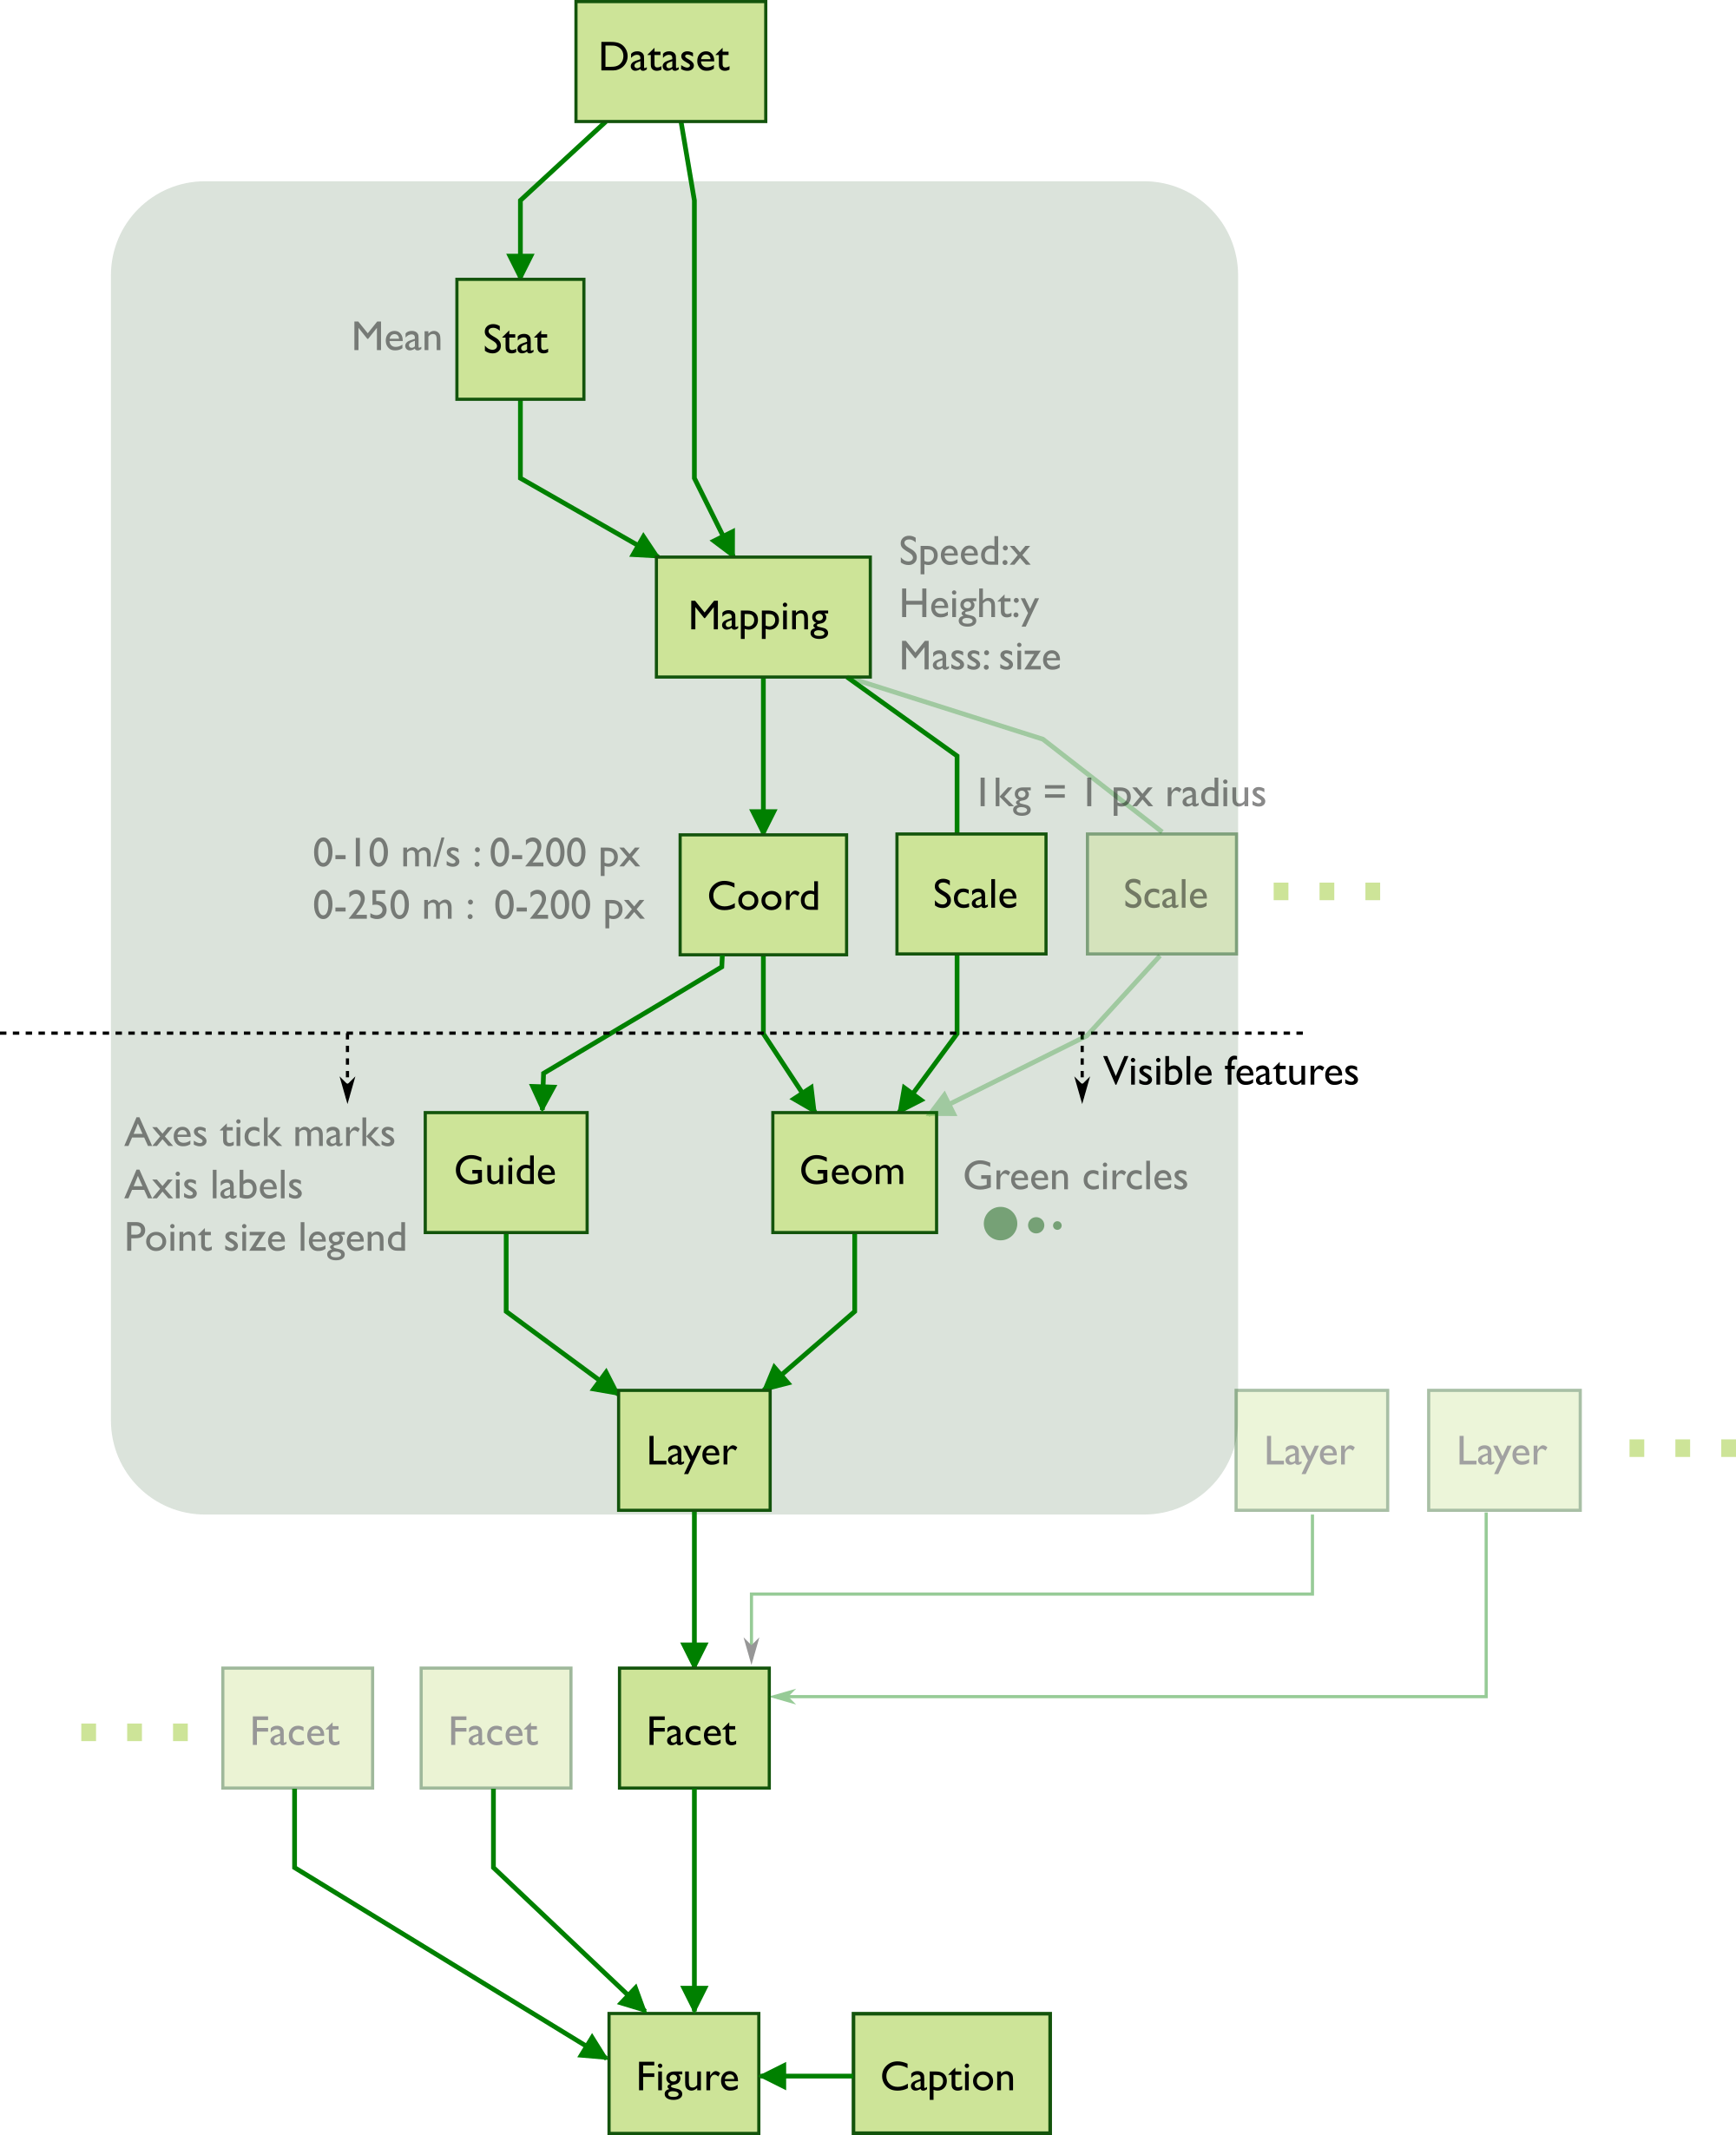
\includegraphics[scale=0.5]{src/2.1 grammar of graphics.png}
    \caption{The Flowchart of layered grammar of graphics.}
\end{figure}

An example of a figure is given below.
\begin{figure}[H]
    \centering
    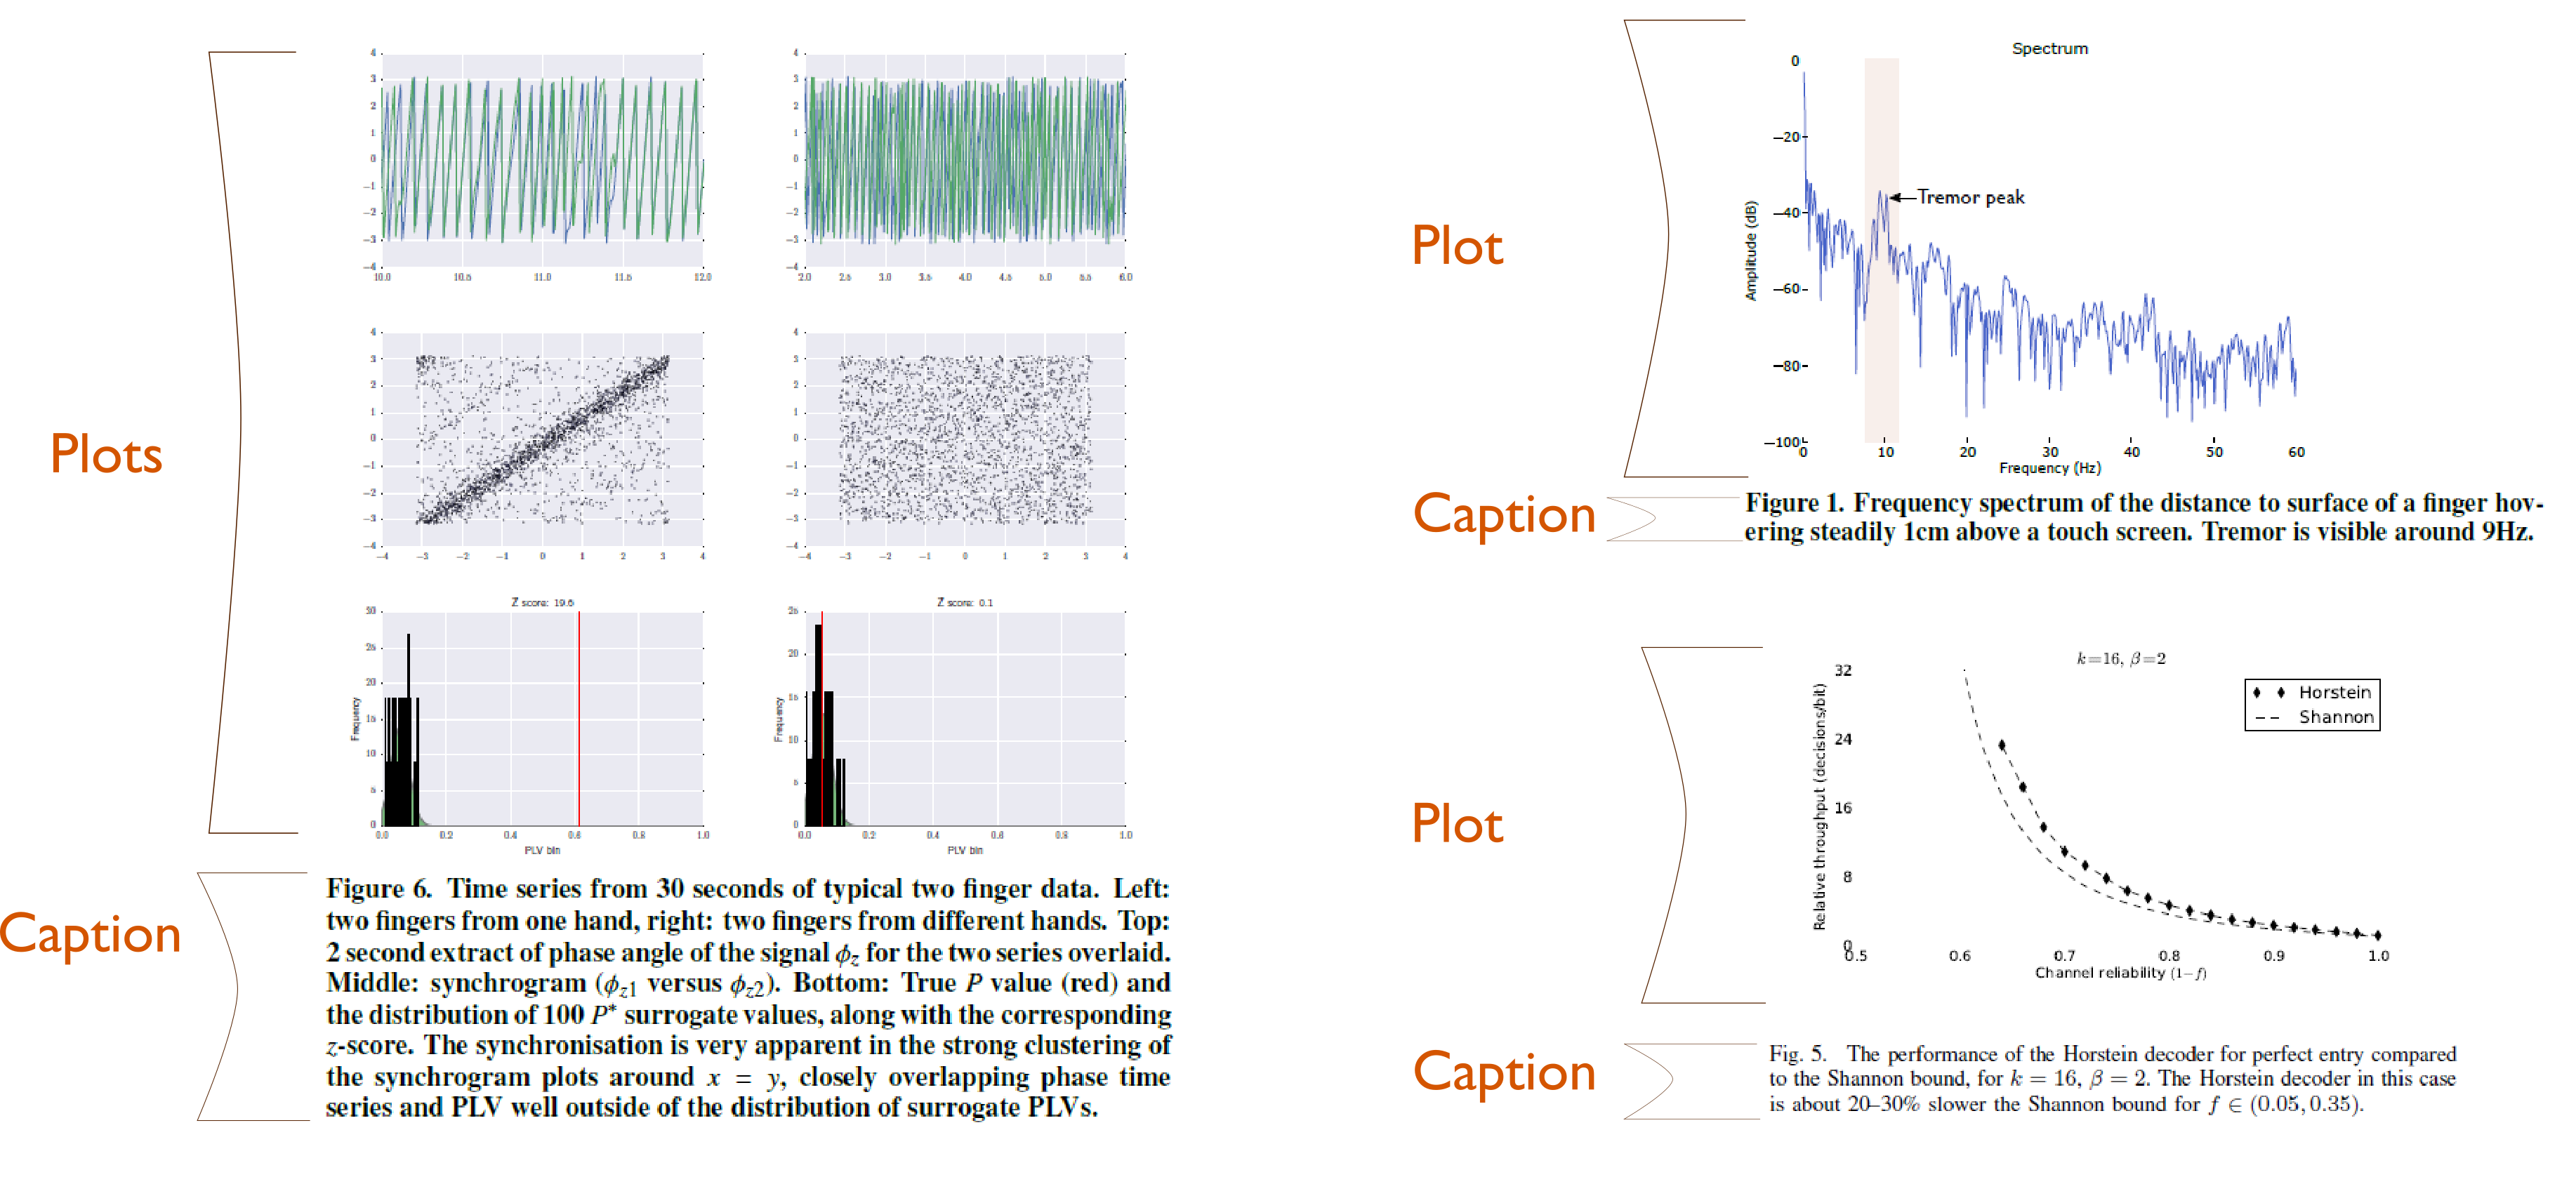
\includegraphics[scale=0.25]{src/2.2 figure examples.png}
    \caption{Examples of multiple figures.}
\end{figure}
\noindent In the graph, the figure on the left has 6 facets; the top right figure has one facet with single layer; the bottom right figure has one facet and two layers.

A plot should have guides to explain how the stats/raw values from the dataset have been mapped to the coordinate system. This includes:
\begin{itemize}
    \item Labelled axes, with units if present. These are part of the guide.
    \item Ticks, which indicate subdivisons of an axis with respect to the units. We can have minor and major ticks in the graph, in both axes. These are also part of the guide.
    \item A legend, to explain what each of the marker/line means (if more than one present). These are guides and help distinguish the different layers.
    \item A title, to explain what the plot is.
\end{itemize}

Moreover, to plot can have:
\begin{itemize}
    \item Grid lines, to help the reader to line the data up-. This is a guide for the coordinate system.
    \item Annotations, to point out relevant features.
\end{itemize}

To display data, plots have geoms. These are geometric objects that represent some element of the data. These include:
\begin{itemize}
    \item lines/curves, which represent continuous functions. They have colour, thickness and style (e.g. dotted, dashed, etc.)
    \item markers, which represent disconnected point. They have colour, size and style.
    \item patches, which represent a shape with an area (e.g. bars in a bar chart). They have colour, size and style.
\end{itemize}

The anatomy of a figure is given below.
\begin{figure}[H]
    \centering
    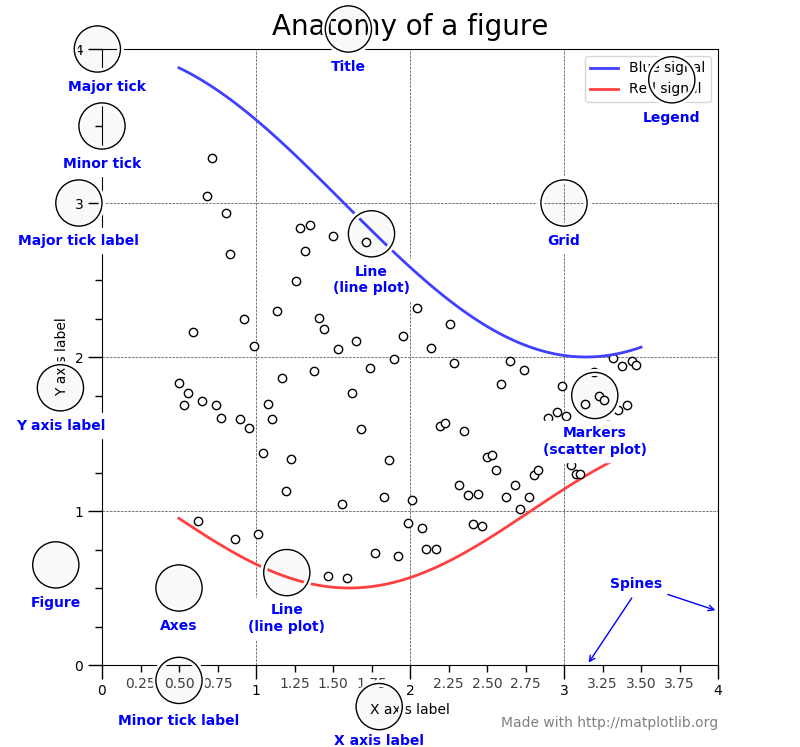
\includegraphics[scale=0.5]{src/2.3 anatomy of a figure.png}
    \caption{The anatomy of a figure}
\end{figure}
\noindent In the figure, we have 3 geoms: one blue line geom, one red line geom, and a point geom. All of these have been plotted on the same coord- they form different layers. There is a legend to distinguish the blue and the red lines, along with tick guides to help identify the $x$ and the $y$ value.

We will use \texttt{matplotlib} for visualisation. An example of a matplotlib graph is given below.
\begin{figure}[H]
    \centering
    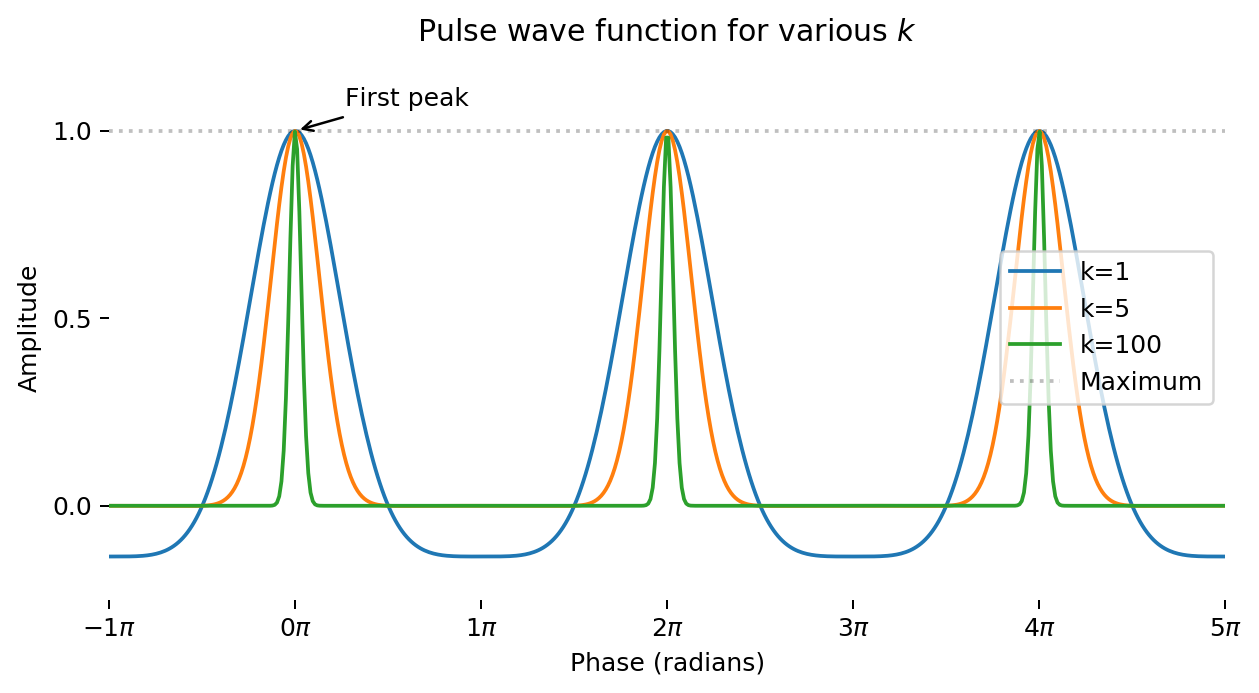
\includegraphics[scale=0.55]{src/2.4 example matplotlib plot.png}
    \caption{A \texttt{matplotlib} plot.}
\end{figure}
\newpage

\section{Simple Plots}
Most of the time, a plot will only have two variables- one independent variable, and one dependent variable, which depends on the independent variable. In a function $y = f(x)$, $x$ is the independent variable, and $y$ is the dependent variable- it depends on the value of $x$. As with the notation, the independent variable is plotted on the $x$-axis, and the dependent variable on the $y$-axis.

For example, assume we have a dataset that compares the number of door head hitting incidents with height. Then, the independent variable is the height, since it is independent of the number of door head hitting incidents. Moreover, the dependent variable is the door head hitting incidents- it depends on the height of the person. In particular, when looking at the dataset, comparing height and the number of incidents, we would expect that as the height increases, the number of door head hitting incident increases.

2D plots are used to visualise two columns of a dataset (or a stat), and maps one to the $x$-axis, and the other to the $y$-axis. The following are some common types of 2D plots:
\begin{itemize}
    \item Scatterplot: a scatterplot marks $(x, y)$ locations with markers. Markers are point geoms. An example is given below.
    \begin{figure}[H]
        \centering
        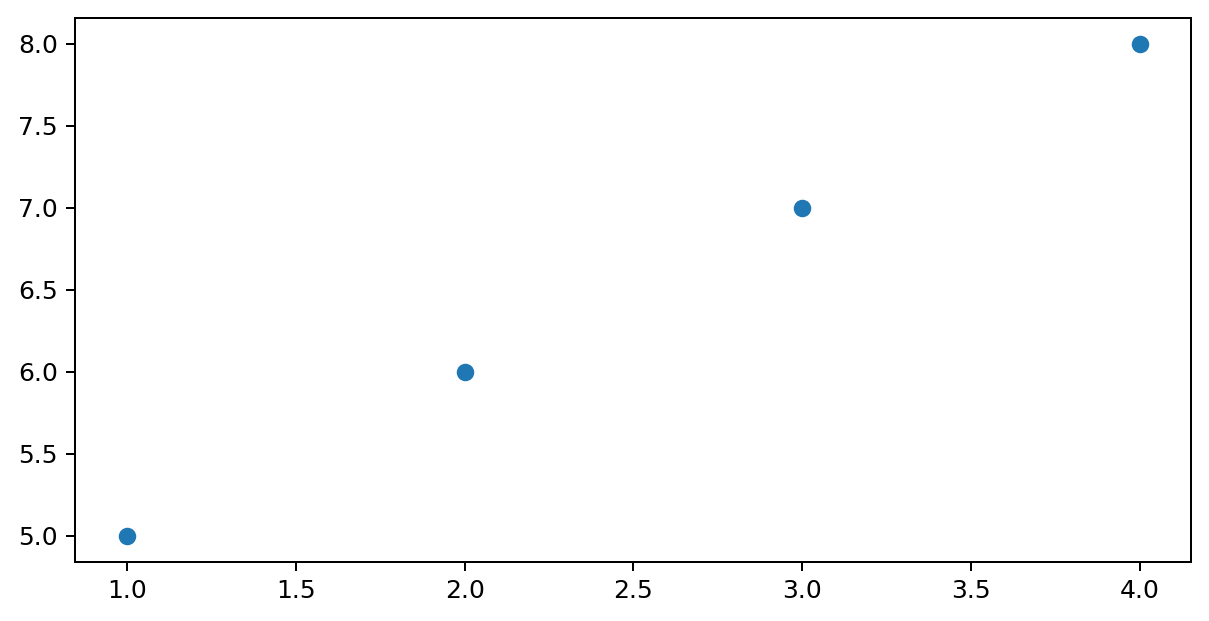
\includegraphics[scale=0.4]{src/2.5 scatterplot example.png}
        \caption{An example of a scatterplot.}
    \end{figure}

    \item Bar chart: for $(x, y)$ in the dataset, it draws bars at $x$ with size proportional to the value of $y$. These are patch geoms. An example is given below.
    \begin{figure}[H]
        \centering
        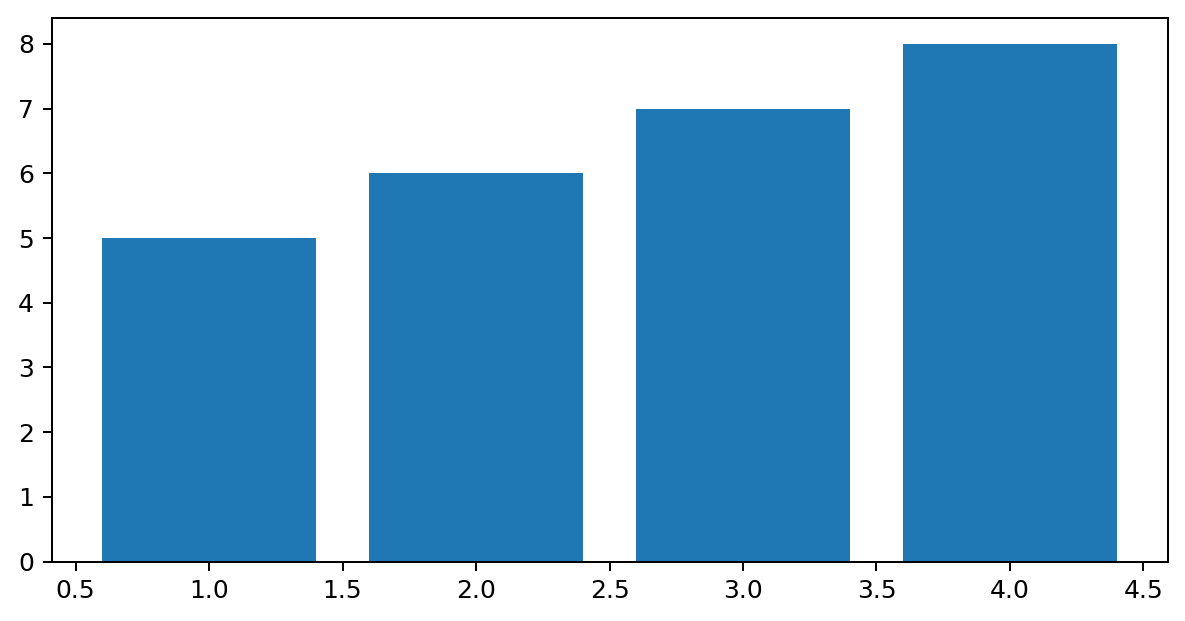
\includegraphics[scale=0.4]{src/2.6 bar chart example.png}
        \caption{An example of a bar chart.}
    \end{figure}

    \item Line plot: draws line segments between the values of $(x, y)$ provided, in the given below. These are line geoms.
    \begin{figure}[H]
        \centering
        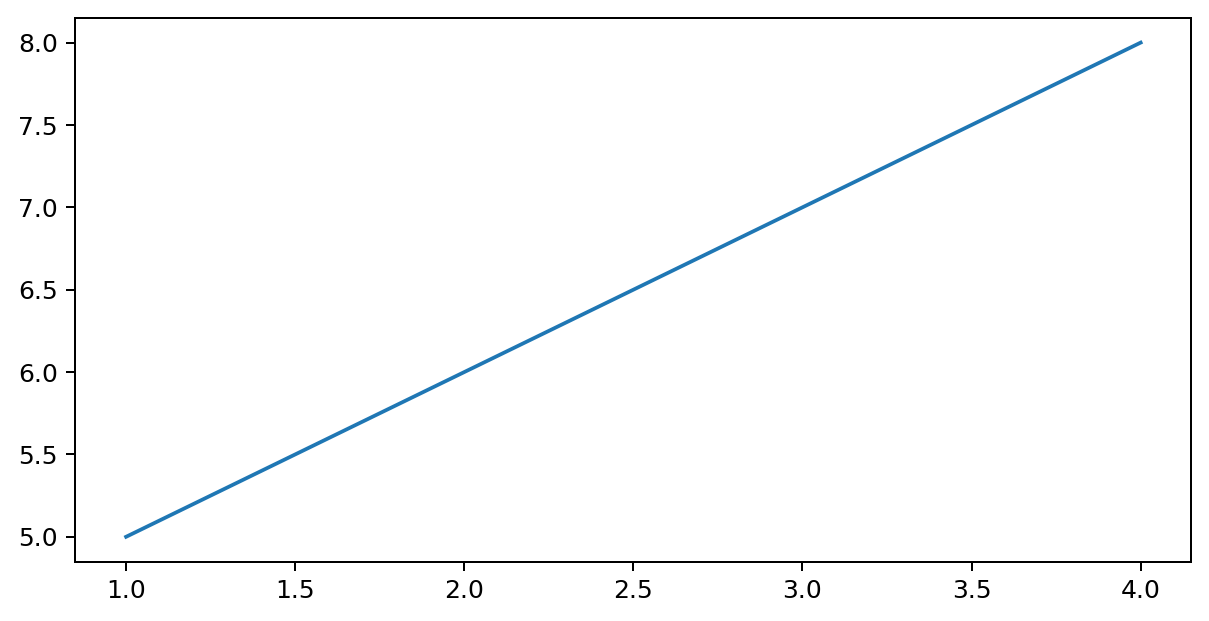
\includegraphics[scale=0.4]{src/2.7 line plot example.png}
        \caption{An example of a line plot.}
    \end{figure}
    We can add markers to the line plot to highlight the actual measurements we observed. These are point geoms.
    \begin{figure}[H]
        \centering
        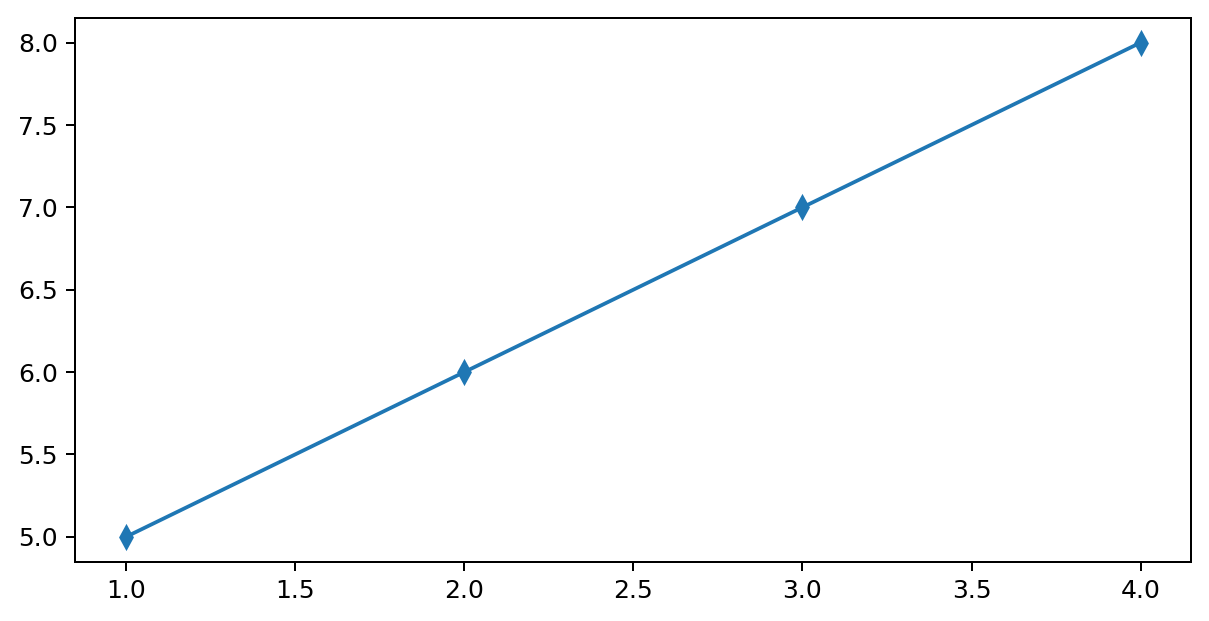
\includegraphics[scale=0.4]{src/2.8 line plot example with markers.png}
        \caption{An example of a line plot with markers.}
    \end{figure}
    This plot has 2 geoms in the same layer- a line geom and a point geom.
    
    \item Ribbon plot- given $(x, y_{\min}, y_{\max})$, plots lines $(x, y_{\min})$ and $(x, y_{\max})$, and covers the area between $y_{\min}$ and $y_{\max}$. These are polygon geoms; the thickness of the ribbon varies with respect to the $x$ value.
    \begin{figure}[H]
        \centering
        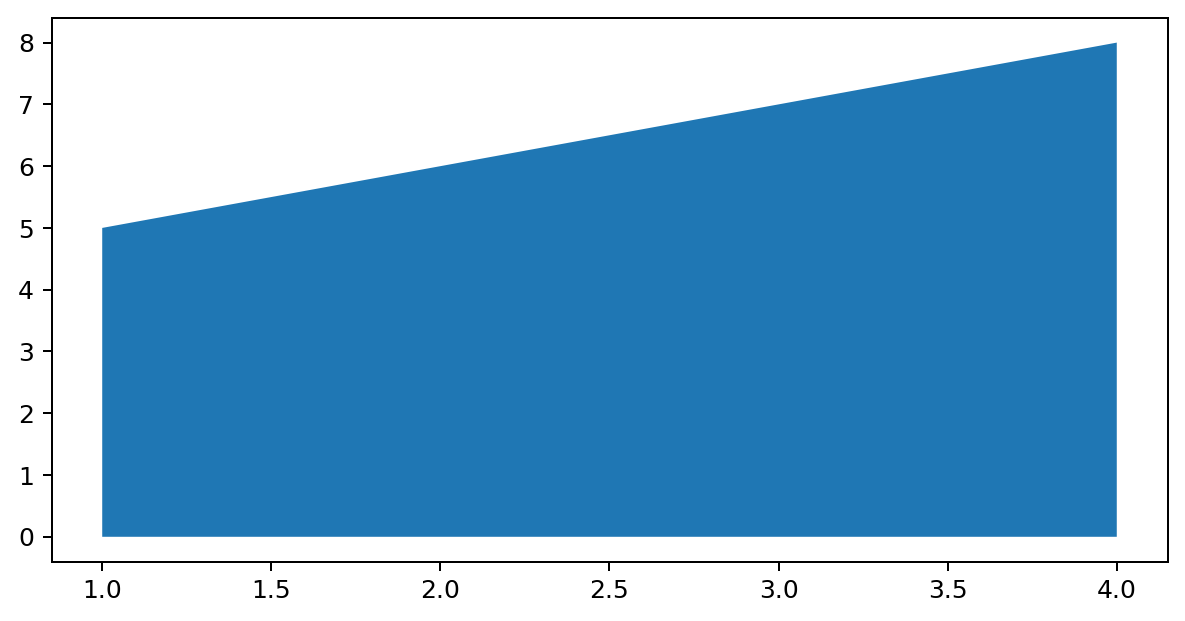
\includegraphics[scale=0.4]{src/2.9 ribbon plot example.png}
        \caption{An example of a ribbon plot.}
    \end{figure}
\end{itemize}
In a layer, we can combine these geoms. For example, we can use:
\begin{itemize}
    \item line geoms for the trend of the data;
    \item point geoms for the raw data; and
    \item area geoms for the uncertainity with the data.
\end{itemize}
An example of the graph is given below.
\begin{figure}[H]
    \centering
    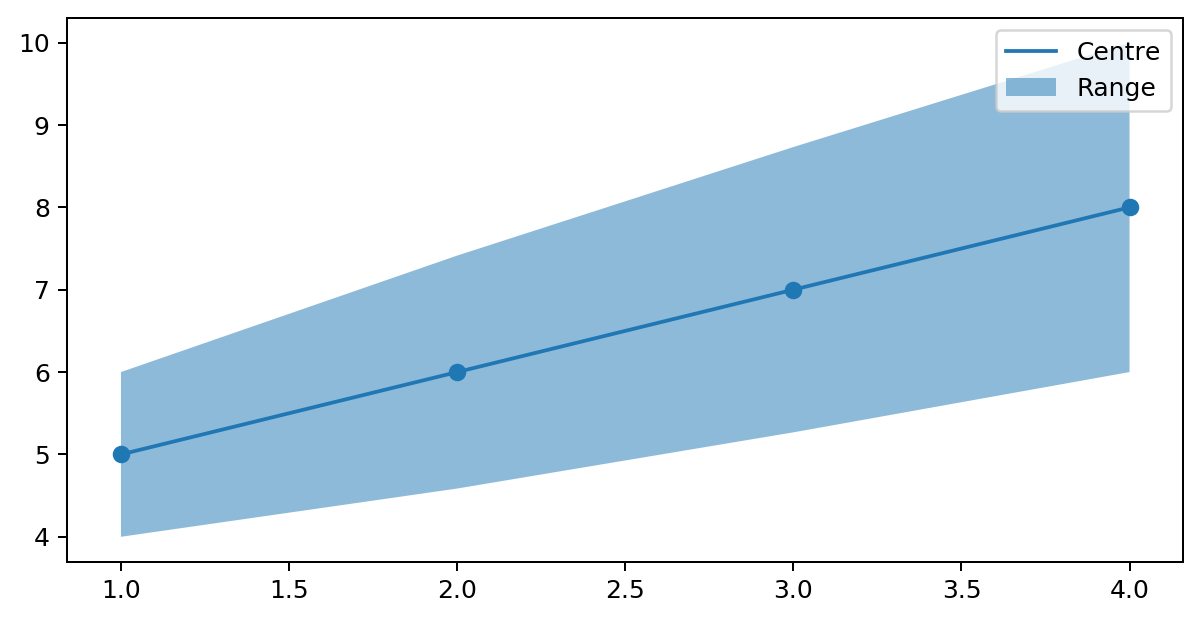
\includegraphics[scale=0.5]{src/2.10 ribbon plot with central line and markers.png}
    \caption{A ribbon plot with central line and markers.}
\end{figure}
\newpage

\section{How to not plot}
We will now look at different examples of visualisation and criticise/improve them. First, assume that we are comparing various doses of vitamin C and how that affects the length of guinea pig teeth length. The vitamin C is given either as a vitamin C tablet, or orange juice.

If we just loaded the data and plotted them as a line graph, carelessly, we could end up with the following graph.
\begin{figure}[H]
    \centering
    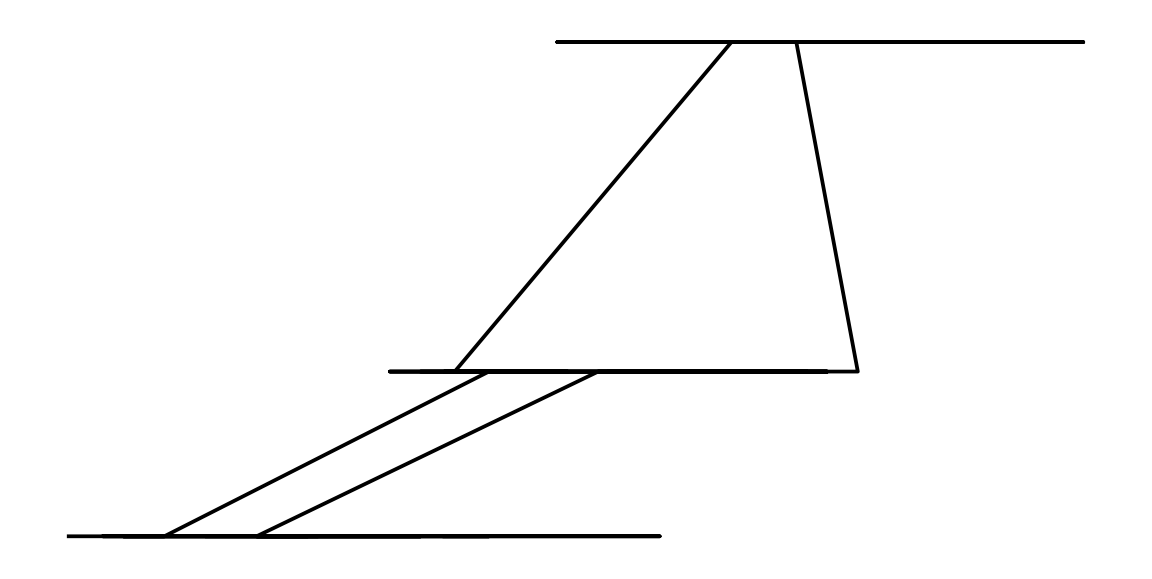
\includegraphics[scale=0.4]{src/2.11 VitC Example Plot 1.png}
    \caption{A bad plot of comparing the effect of vitamin C on guinea pig tooth growth.}
\end{figure}
This is a bad plot. In particular,
\begin{itemize}
    \item It has no guides- no axis, no ticks, no labels, no units, no title and no legend.
    \item It has bad coords- the dependent variable is on the $x$-axis, and the independent on the $y$-axis.
    \item It has bad mappings- there is no way to distinguish the two sets of data (vitamin C and orange juice).
    \item It has bad geoms- we have plotted lines even though the data is not continuous.
\end{itemize}

We can improve this plot by using scatterplots and distinguishing the two datasets.
\begin{figure}[H]
    \centering
    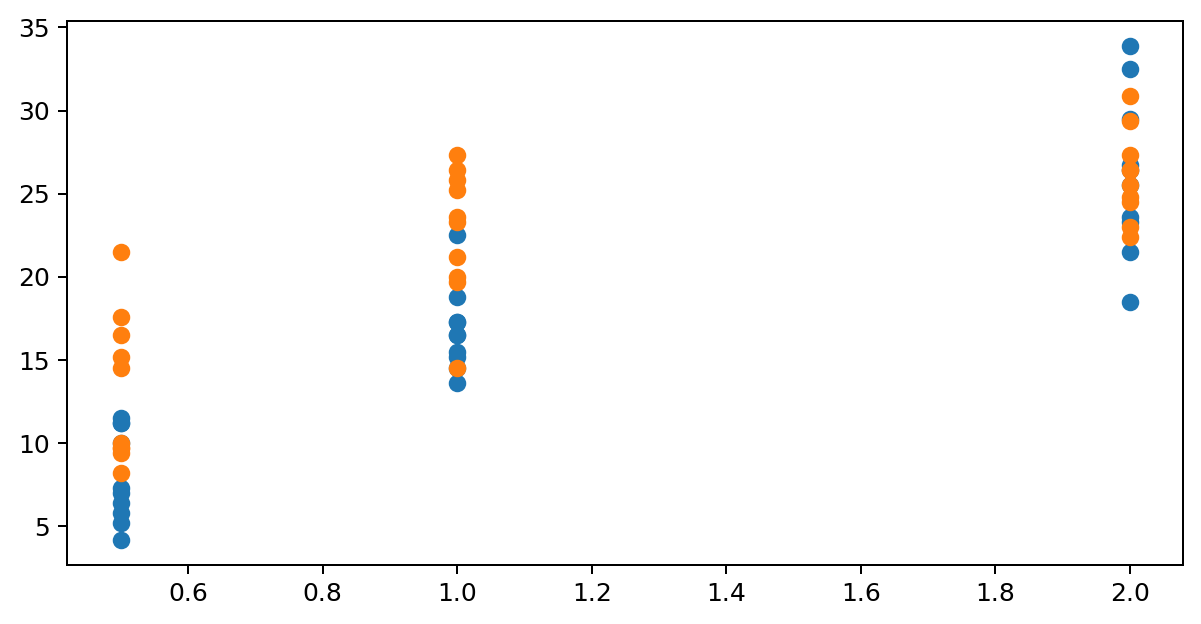
\includegraphics[scale=0.5]{src/2.12 VitC Example Plot 2.png}
    \caption{A slightly better plot of comparing the effect of vitamin C on guinea pig tooth growth.}
\end{figure}
Now, it has:
\begin{itemize}
    \item guides- the $x$ and the $y$-values are labelled;
    \item good coords- the dependent variable is on the $y$-axis, and the independent on the $x$-axis;
    \item good geoms- scatterplot is better suited in this case than line plots since the data is not continuous; and
    \item good mapping- it is possible to distinguish the two datasets (even though we do not know which set of data corresponds to which colour).
\end{itemize}

Next, we add some labels and guides to the data.
\begin{figure}[H]
    \centering
    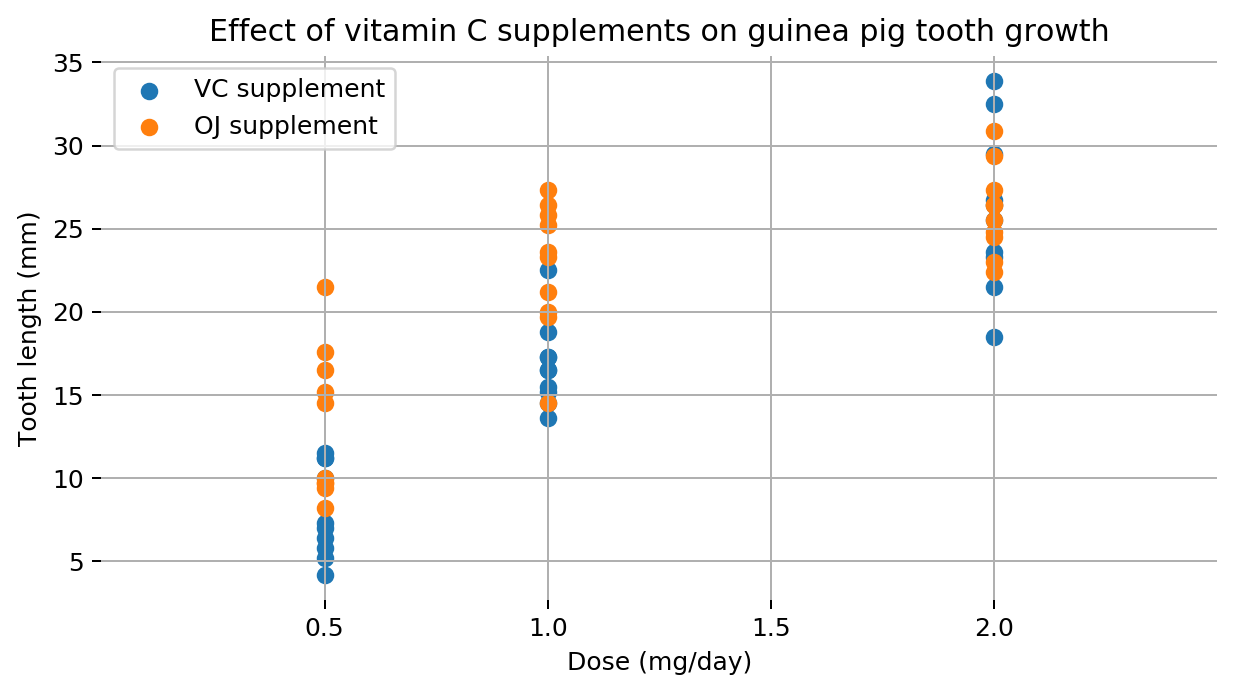
\includegraphics[scale=0.5]{src/2.13 VitC Example Plot 3.png}
    \caption{A good plot of comparing the effect of vitamin C on guinea pig tooth growth.}
\end{figure}
Now, we have added guides. In particular:
\begin{itemize}
    \item the plot has a title;
    \item the axes are labelled, with units;
    \item the legend identifies the two layers;
    \item the grid helps with reading the coordinates;
    \item the $x$-ticks are placed correctly (they are precisely where the data is); and
    \item the $y$-ticks extend to the origin.
\end{itemize}

Also, we can add $x$ and $y$ limits so that the bottom left value is the origin.
\begin{figure}[H]
    \centering
    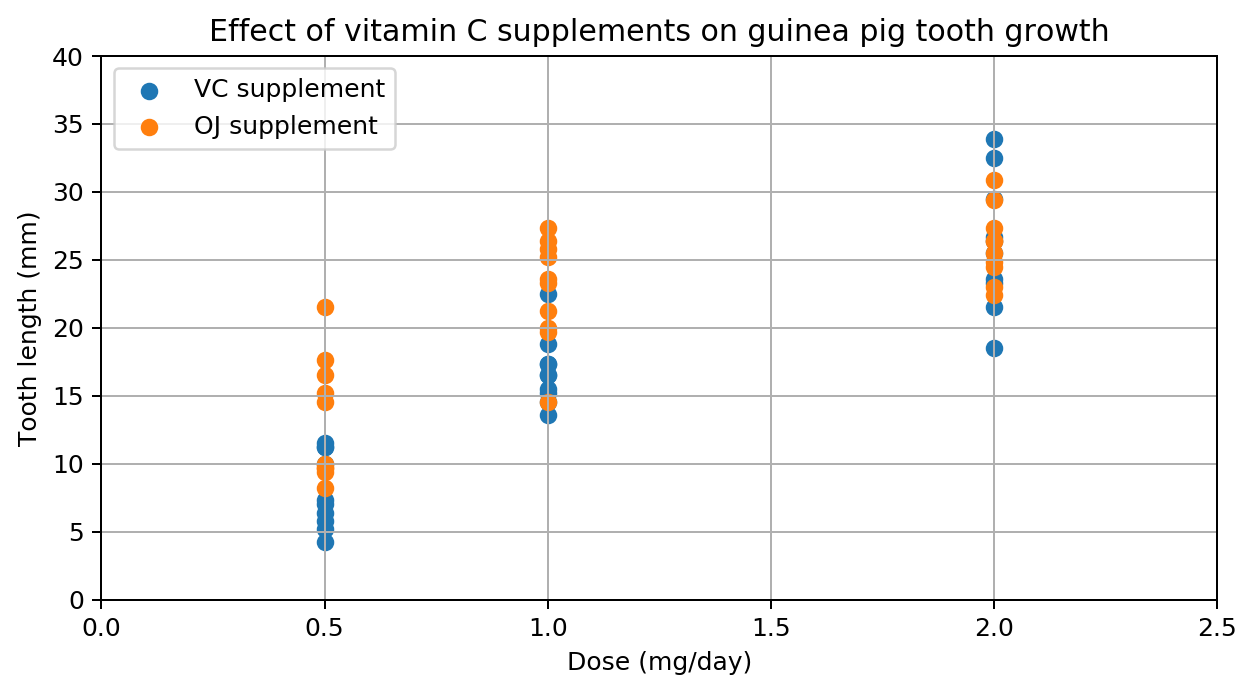
\includegraphics[scale=0.5]{src/2.14 VitC Example Plot 4.png}
    \caption{Another good plot of comparing the effect of vitamin C on guinea pig tooth growth.}
\end{figure}
We should always aim to start at the origin; not starting at the origin can make the data more deceiving. Nonetheless, it should not be done if the plot cannot be visualised clearly after the transformation.

At this point, the two views (vitamin C and orange juice) have been plotted on the same coord as different layers. We can also plot them on different facets, as shown below.
\begin{figure}[H]
    \centering
    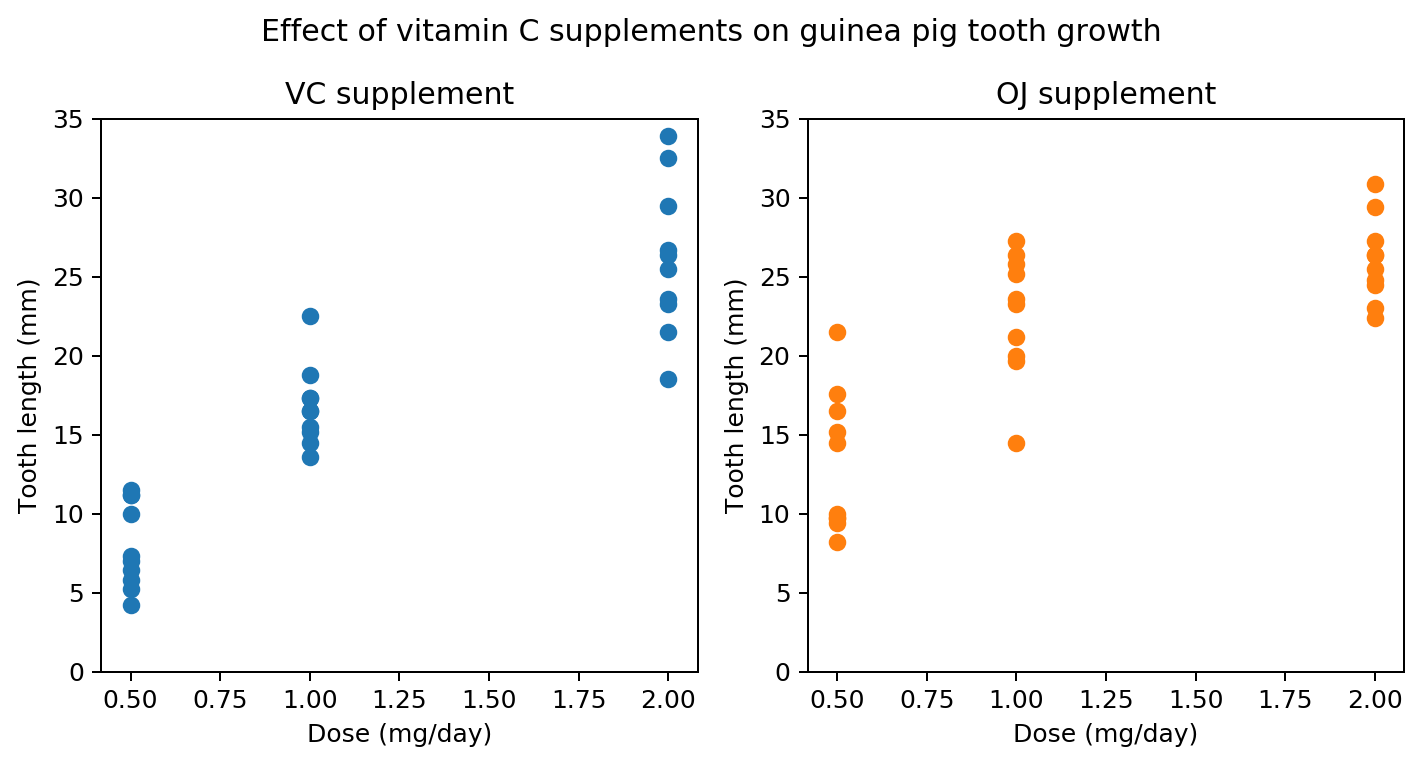
\includegraphics[scale=0.5]{src/2.15 VitC Example Plot 5.png}
    \caption{A faceted plot of comparing the effect of vitamin C on guinea pig tooth growth.}
\end{figure}
\newpage

\section{Multiple visualisations of a dataset}
Now, we will look at multiple visualisations of a dataset with another example. Assume we have a dataset that gives the gas usage in the UK from 1960-1986, one every 3 months. We can create a simple line graph out of it, with markers to show raw data.
\begin{figure}[H]
    \centering
    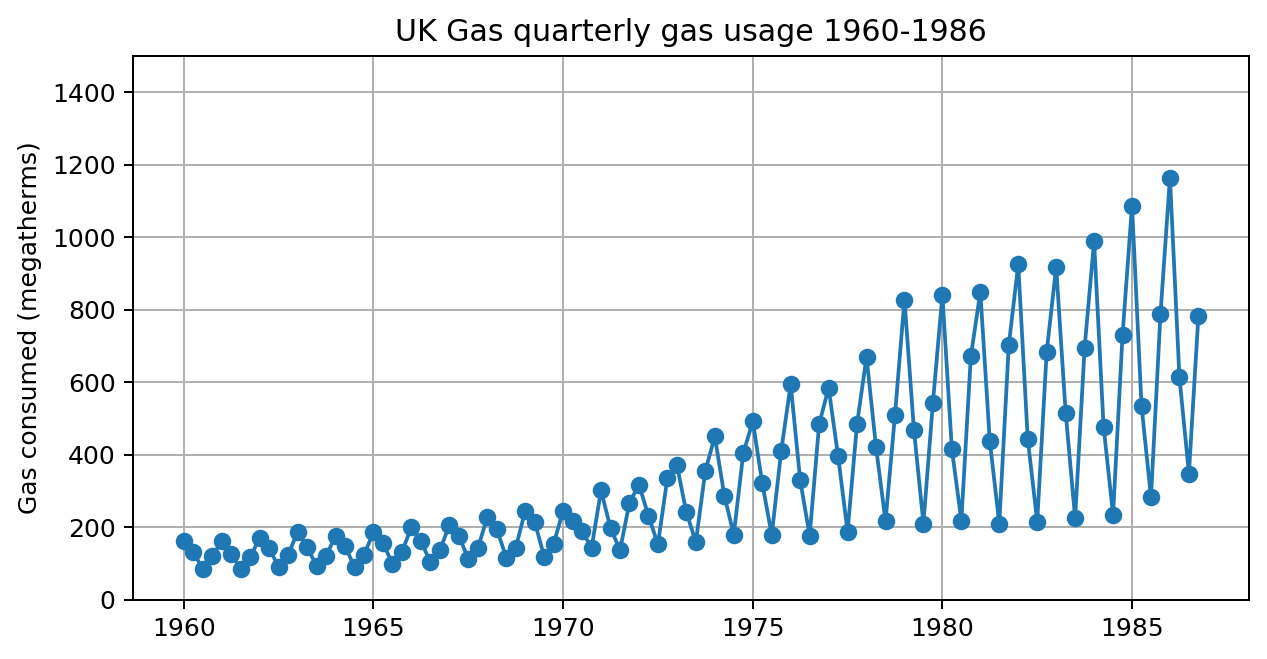
\includegraphics[scale=0.4]{src/2.16 Gas Example Plot 1.png}
    \caption{Gas usage in the UK, 1960-1986.}
\end{figure}
\noindent We can simplify this graph by using the general pattern and smoothening the curve, e.g. using a 3 year running mean. This is a stat.
\begin{figure}[H]
    \centering
    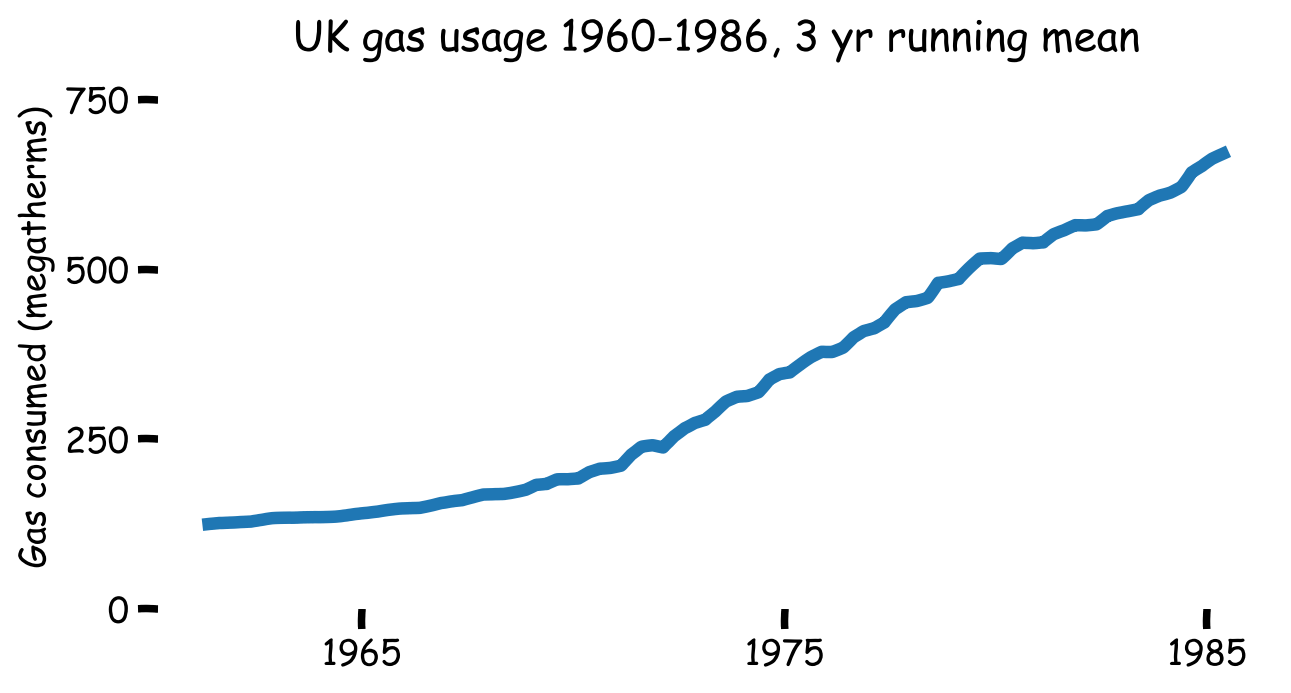
\includegraphics[scale=0.4]{src/2.17 Gas Example Plot 2.png}
    \caption{Gas usage in the UK, 1960-1986, 3 year running mean.}
\end{figure}
\noindent We can also split the data into multiple layers, breaking it with respect to the seasons.
\begin{figure}[H]
    \centering
    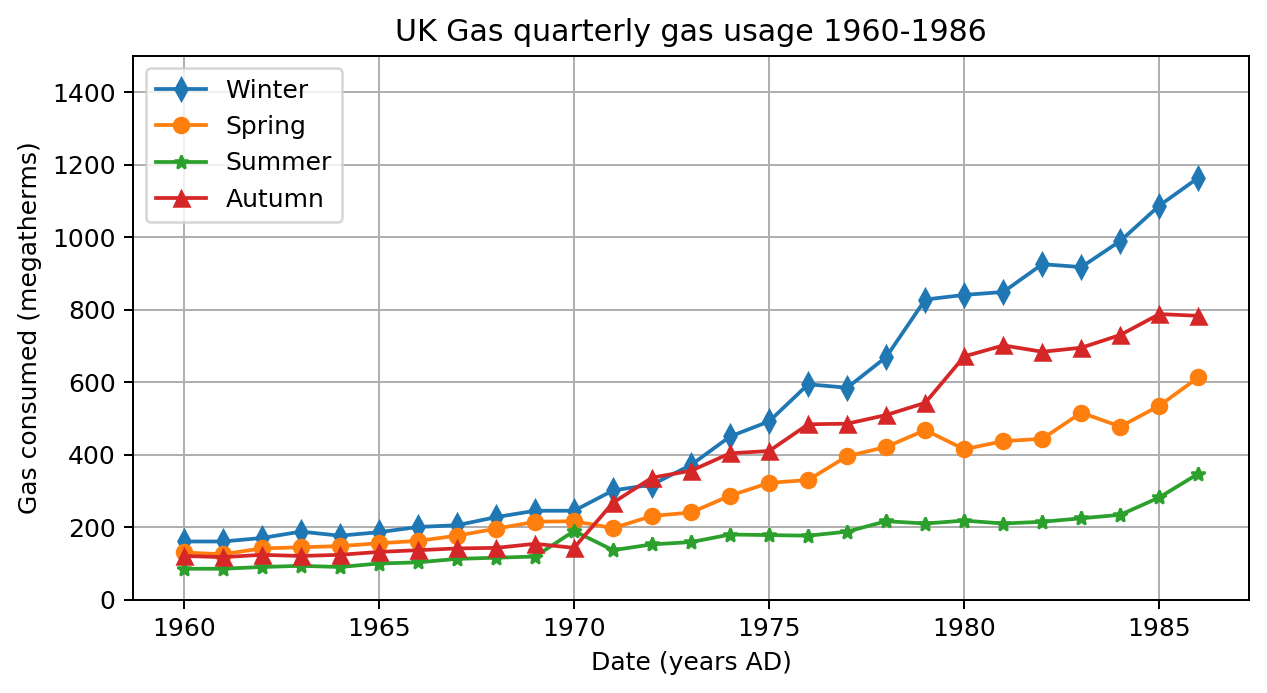
\includegraphics[scale=0.4]{src/2.18 Gas Example Plot 3.png}
    \caption{Gas usage in the UK, 1960-1986, split by quarters.}
\end{figure}
\newpage

\noindent Instead of a layered figure, we can also use a faceted figure.
\begin{figure}[H]
    \centering
    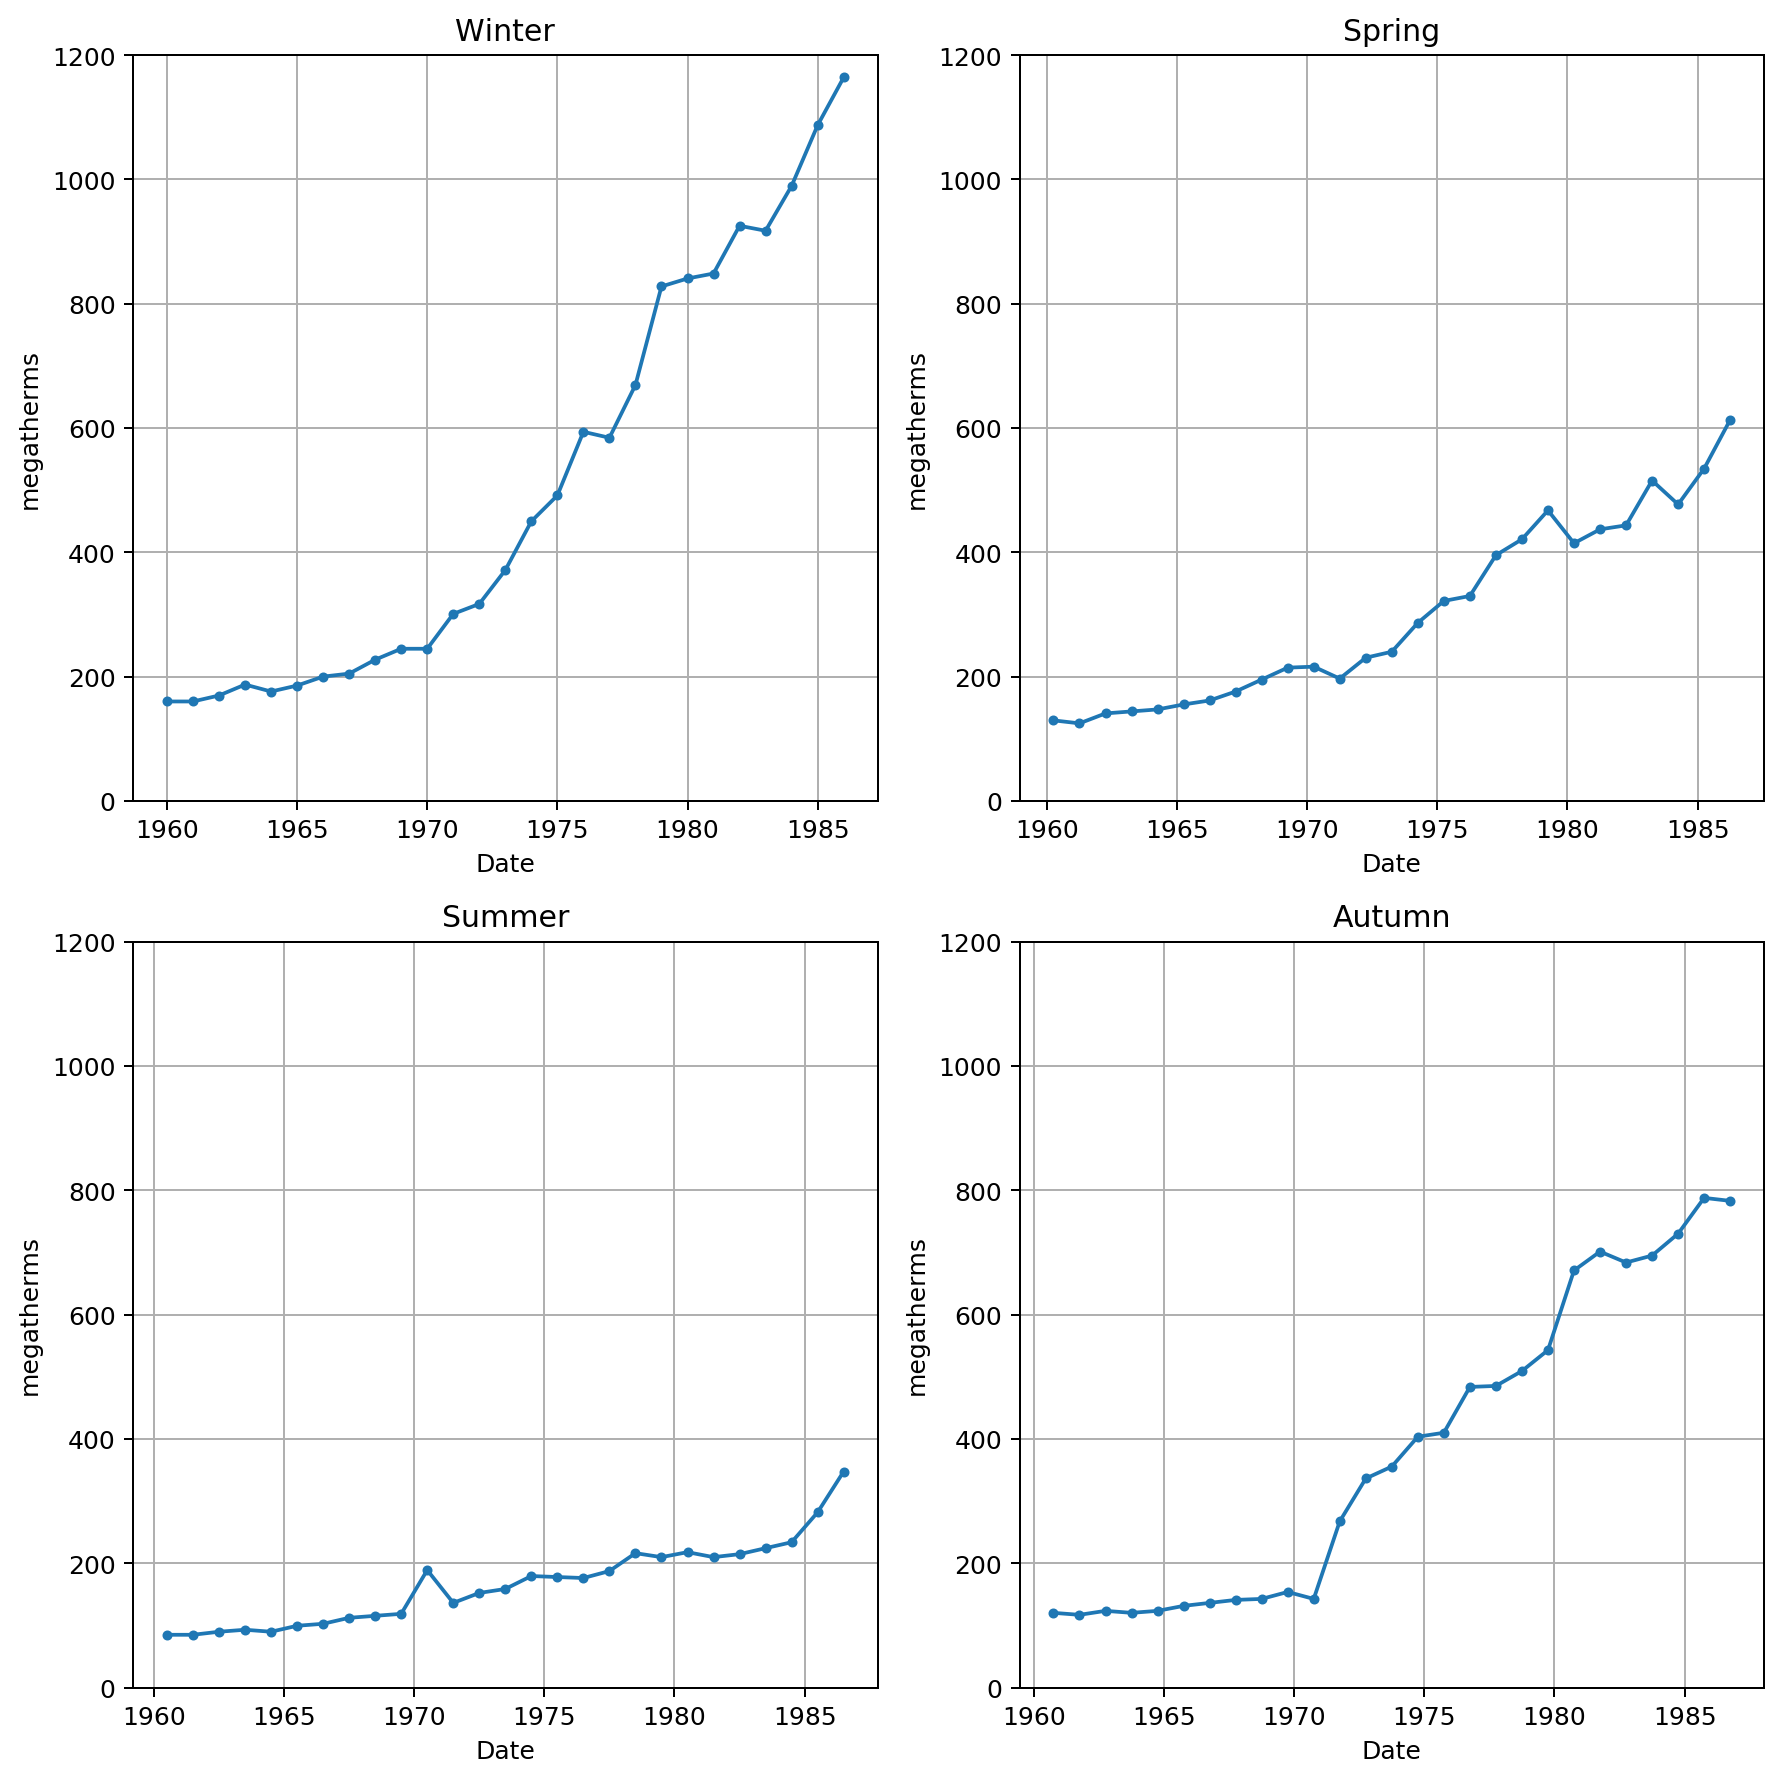
\includegraphics[scale=0.4]{src/2.19 Gas Example Plot 4.png}
    \caption{Gas usage in the UK, 1960-1986, split by quarters, in a faceted figure.}
\end{figure}
\noindent By using the same axis scale in the 4 plots, comparing each plot becomes easy. We can also transform the plot into showing variation among the years for each season in a layered plot.
\begin{figure}[H]
    \centering
    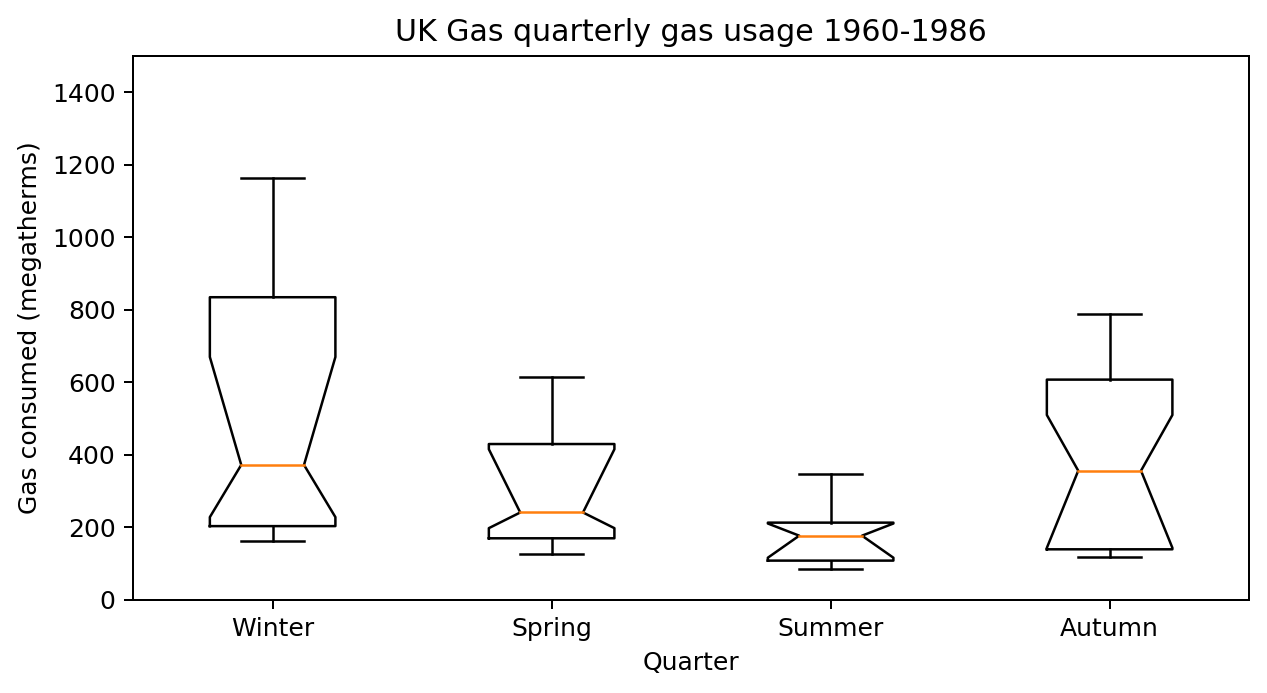
\includegraphics[scale=0.4]{src/2.20 Gas Example Plot 5.png}
    \caption{Gas usage in the UK, 1960-1986, split by quarters, with error bars and mean.}
\end{figure}
\noindent We can also use a ribbon plot to show the mean and the range for each year.
\begin{figure}[H]
    \centering
    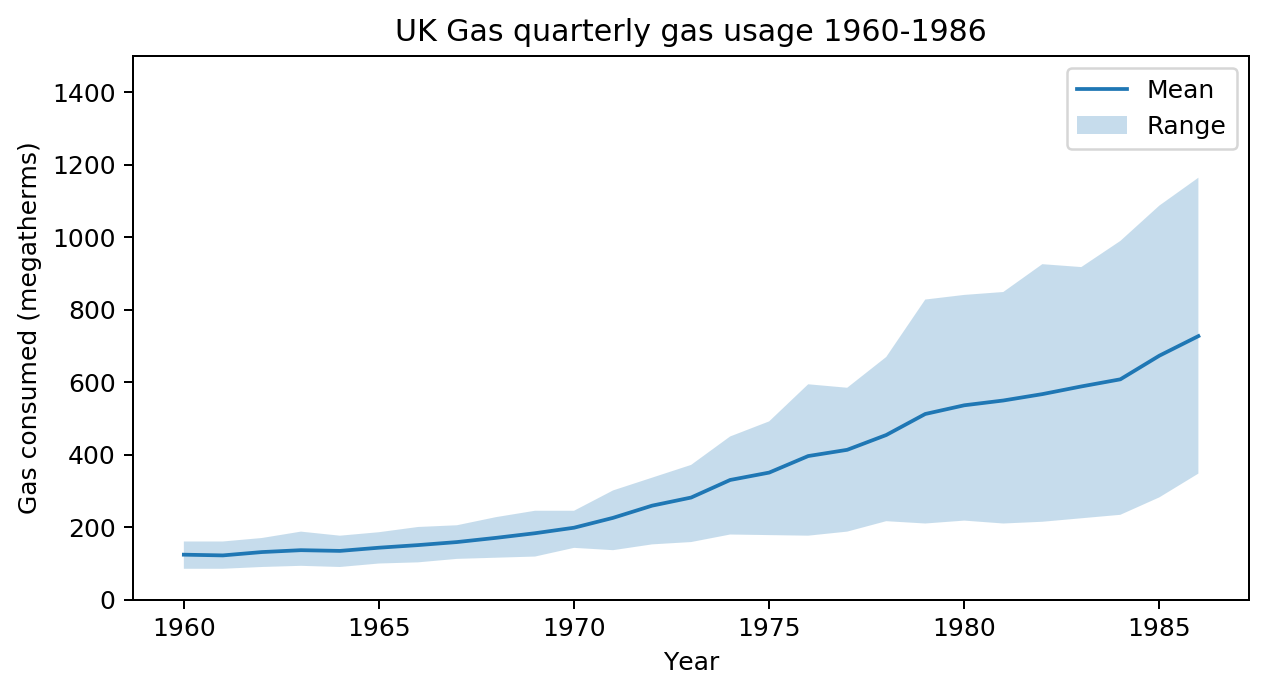
\includegraphics[scale=0.4]{src/2.21 Gas Example Plot 6.png}
    \caption{Gas usage in the UK, 1960-1986, split by quarters, as a ribbon plot with mean and range.}
\end{figure}
\noindent Instead of a ribbon plot, we can use a scatter plot to show the maximum and minimum usage in each year against the median consumption.
\begin{figure}[H]
    \centering
    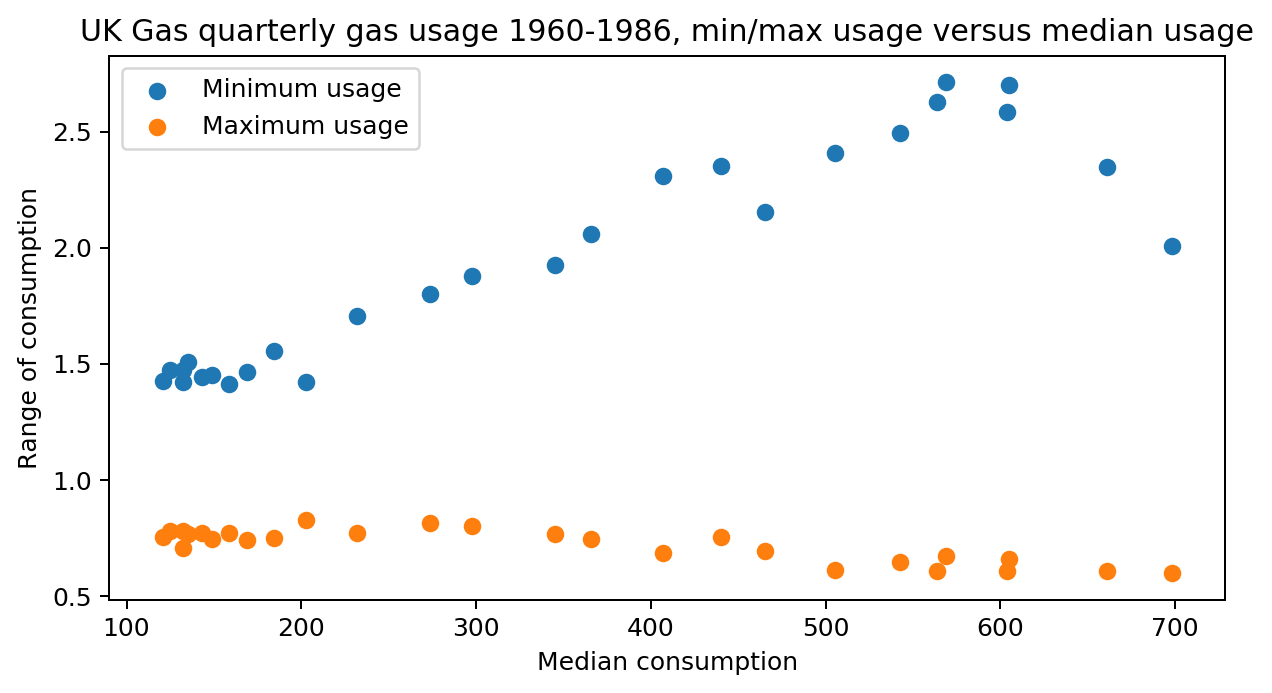
\includegraphics[scale=0.4]{src/2.22 Gas Example Plot 7.png}
    \caption{Gas usage in the UK, 1960-1986, split by quarters, as a scatter plot with minimum and maximum.}
\end{figure}
\noindent Finally, we can produce a cumulative line graph to show the increase in CO2 product. In this case, we are plotting a stat instead of the dataset.
\begin{figure}[H]
    \centering
    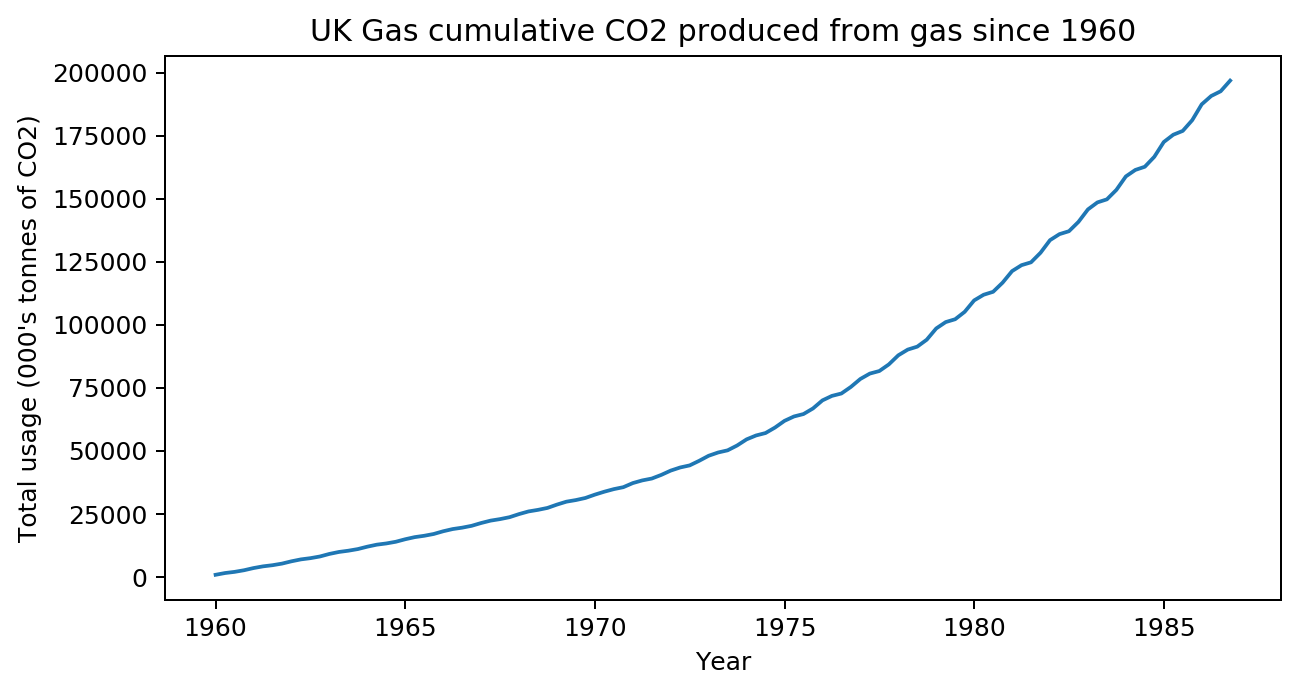
\includegraphics[scale=0.5]{src/2.23 Gas Example Plot 8.png}
    \caption{UK Gas cumulative CO2 produced from gas since 1960.}
\end{figure}
\newpage

\section{Stats}
A stat is a statistic of the dataset, i.e. a transformation of the data. It is used to summarise the data. Common examples are:
\begin{itemize}
    \item aggregation summary statistics, e.g. central tendency (i.e. mean and median), deviation (i.e. standard deviation, max/min, interquartile range);
    \item bining operations, e.g. characterising the data into discrete bins and counting the number of elements in each bin;
    \item smoothing and regression, e.g. approximating functions to datasets, such as linear regression- fitting a line through data.
\end{itemize}

\subsection{Histograms}
Histogram combine binning operation (a stat) and 2D bar chart (a geom). They count the number of values that fall in the given range. We can visualise how the data is distributed across the bins. The bars within the histogram do not have spaces- the bins represent continguous division of the input space. An example of a histogram is given below.
\begin{figure}[H]
    \centering
    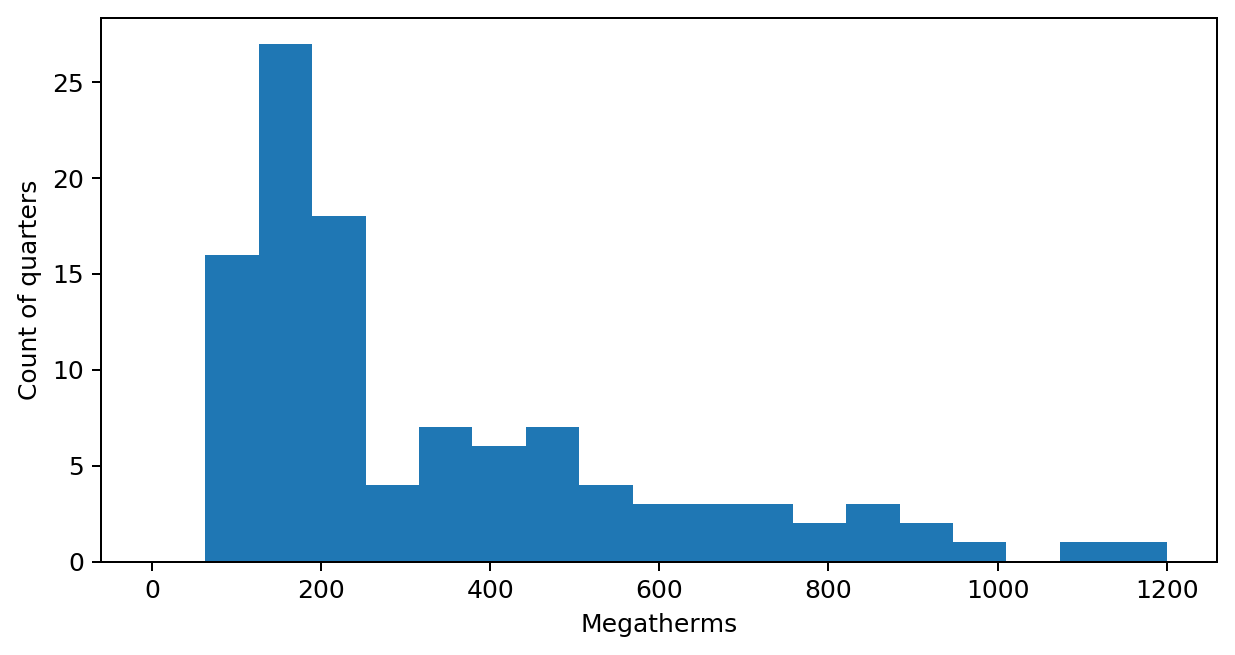
\includegraphics[scale=0.4]{src/2.24 Gas Example Plot 9.png}
    \caption{A histogram from the previous example.}
\end{figure}
\noindent We show how the histogram counts values in bins.
\begin{figure}[H]
    \centering
    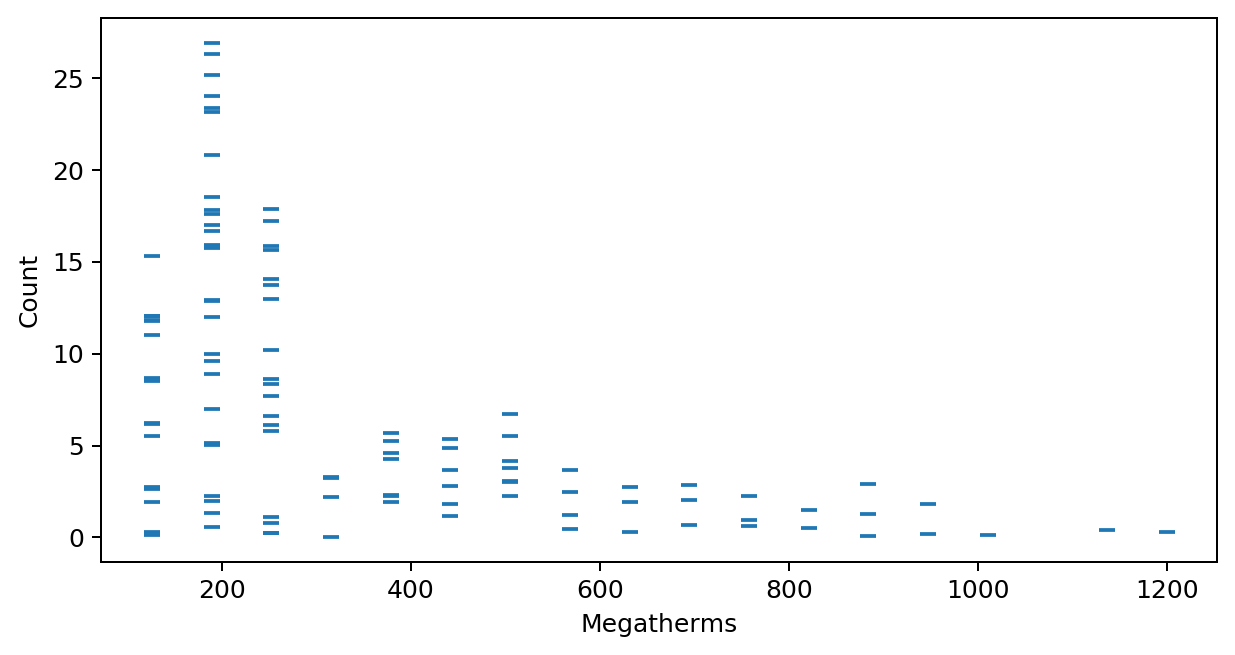
\includegraphics[scale=0.4]{src/2.25 Gas Example Plot 10.png}
    \caption{An illustration of how the histogram counts values in bins.}
\end{figure}
The display of a histogram depends on the choice of the bins. If there are too many bins, the count for  most of the values will be low- it will be difficult to see the trend of the data.
\begin{figure}[H]
    \centering
    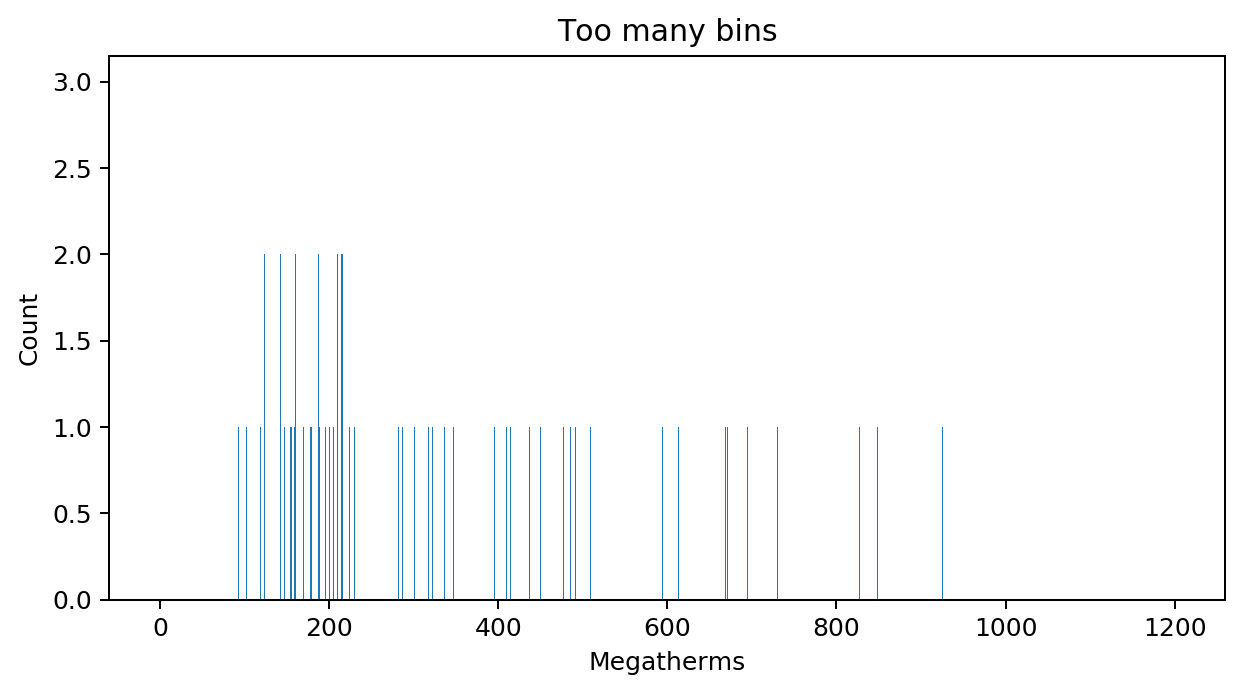
\includegraphics[scale=0.4]{src/2.26 Gas Example Plot 11.png}
    \caption{A histogram with too many bins.}
\end{figure}
\noindent Instead, if there are too few bins, the count for most of the values will be high- the data will be smoothened and details will be lost.
\begin{figure}[H]
    \centering
    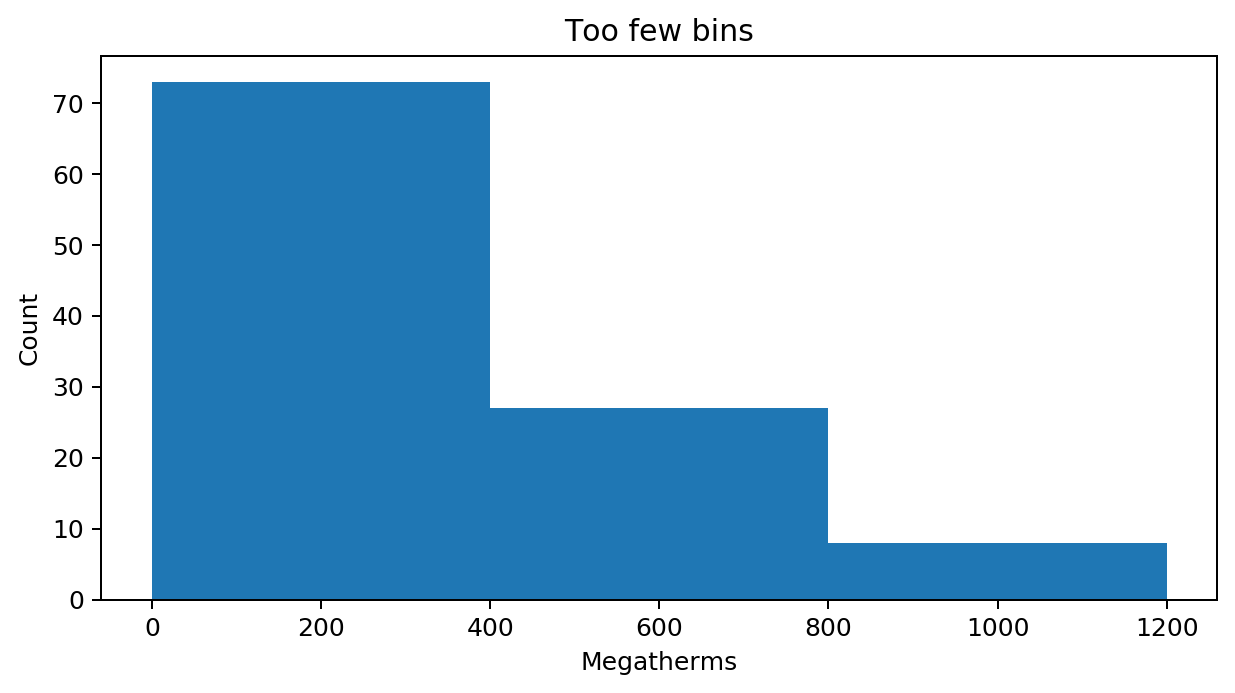
\includegraphics[scale=0.4]{src/2.27 Gas Example Plot 12.png}
    \caption{A histogram with too few bins.}
\end{figure}
\noindent Also, if the bins are badly chosen, then they will not capture the meaningful part of the data; many of the bins will be empty.
\begin{figure}[H]
    \centering
    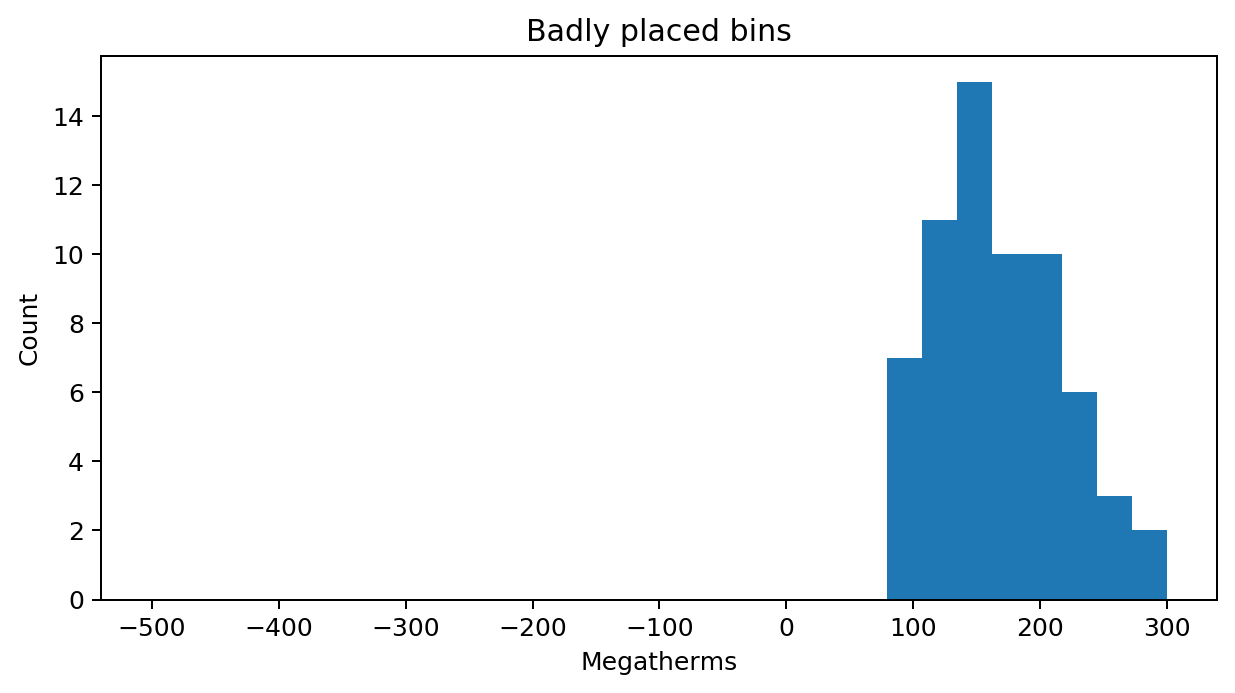
\includegraphics[scale=0.4]{src/2.28 Gas Example Plot 13.png}
    \caption{A histogram with badly placed bins.}
\end{figure}
We can use binning in multiple dimensions as well, though it is difficult to grasp the data in that case.
\begin{figure}[H]
    \centering
    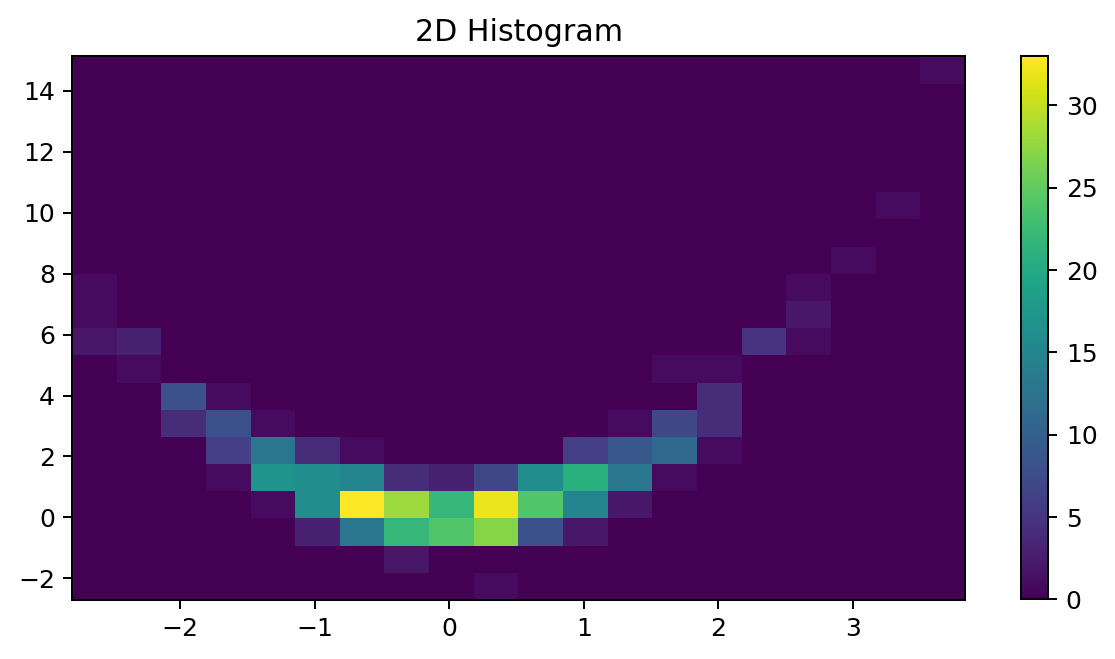
\includegraphics[scale=0.5]{src/2.29 2D Histogram.png}
    \caption{A histogram with badly placed bins.}
\end{figure}

\subsection{Ranking Operations}
For a 1D vector dataset, we can plot it against its rank within the array. The stat here is conversion from the value to the rank.
\begin{figure}[H]
    \centering
    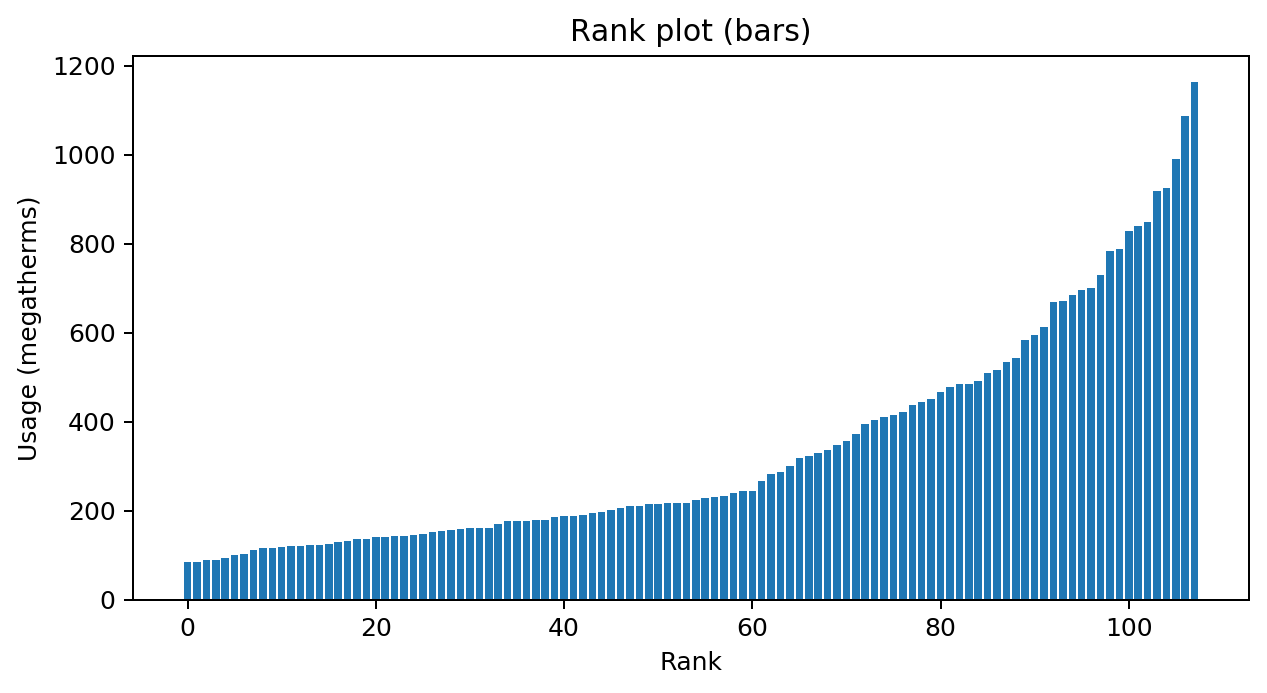
\includegraphics[scale=0.4]{src/2.30 Gas Example Plot 14.png}
    \caption{An example of a rank plot.}
\end{figure}
\noindent In the plot above, we have sorted the usage of gas per quarter, and plotted it against its rank- the index it has in the sorted array. The rank plot can be a scatterplot as well.
\begin{figure}[H]
    \centering
    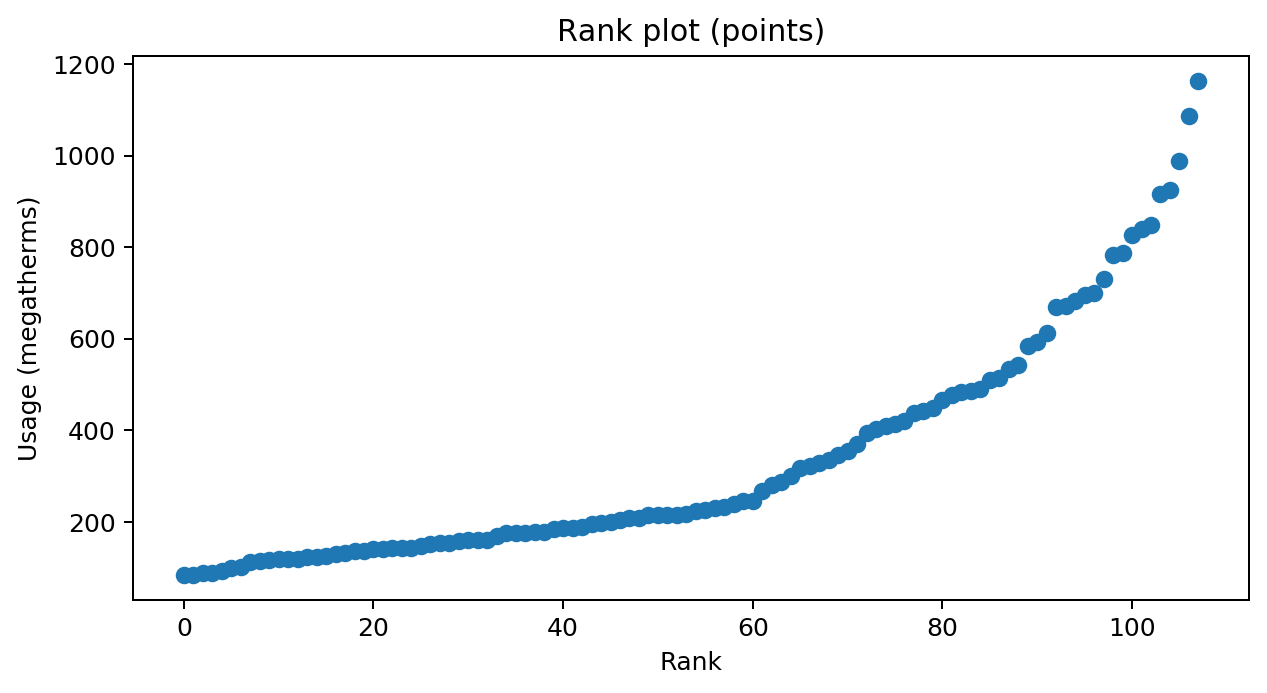
\includegraphics[scale=0.4]{src/2.31 Gas Example Plot 15.png}
    \caption{A scatterplot version rank plot.}
\end{figure}

\subsection{Aggregate Summaries}
It is common to show the range of data (e.g. showing the min/max, standard deviation or the interquartile range). These are often ranges of groupings of the data (e.g. conditions in the experiment). Below is a faceted view of the mean, standard deviation, min, max and center of range, and median of the gas example.
\begin{figure}[H]
    \centering
    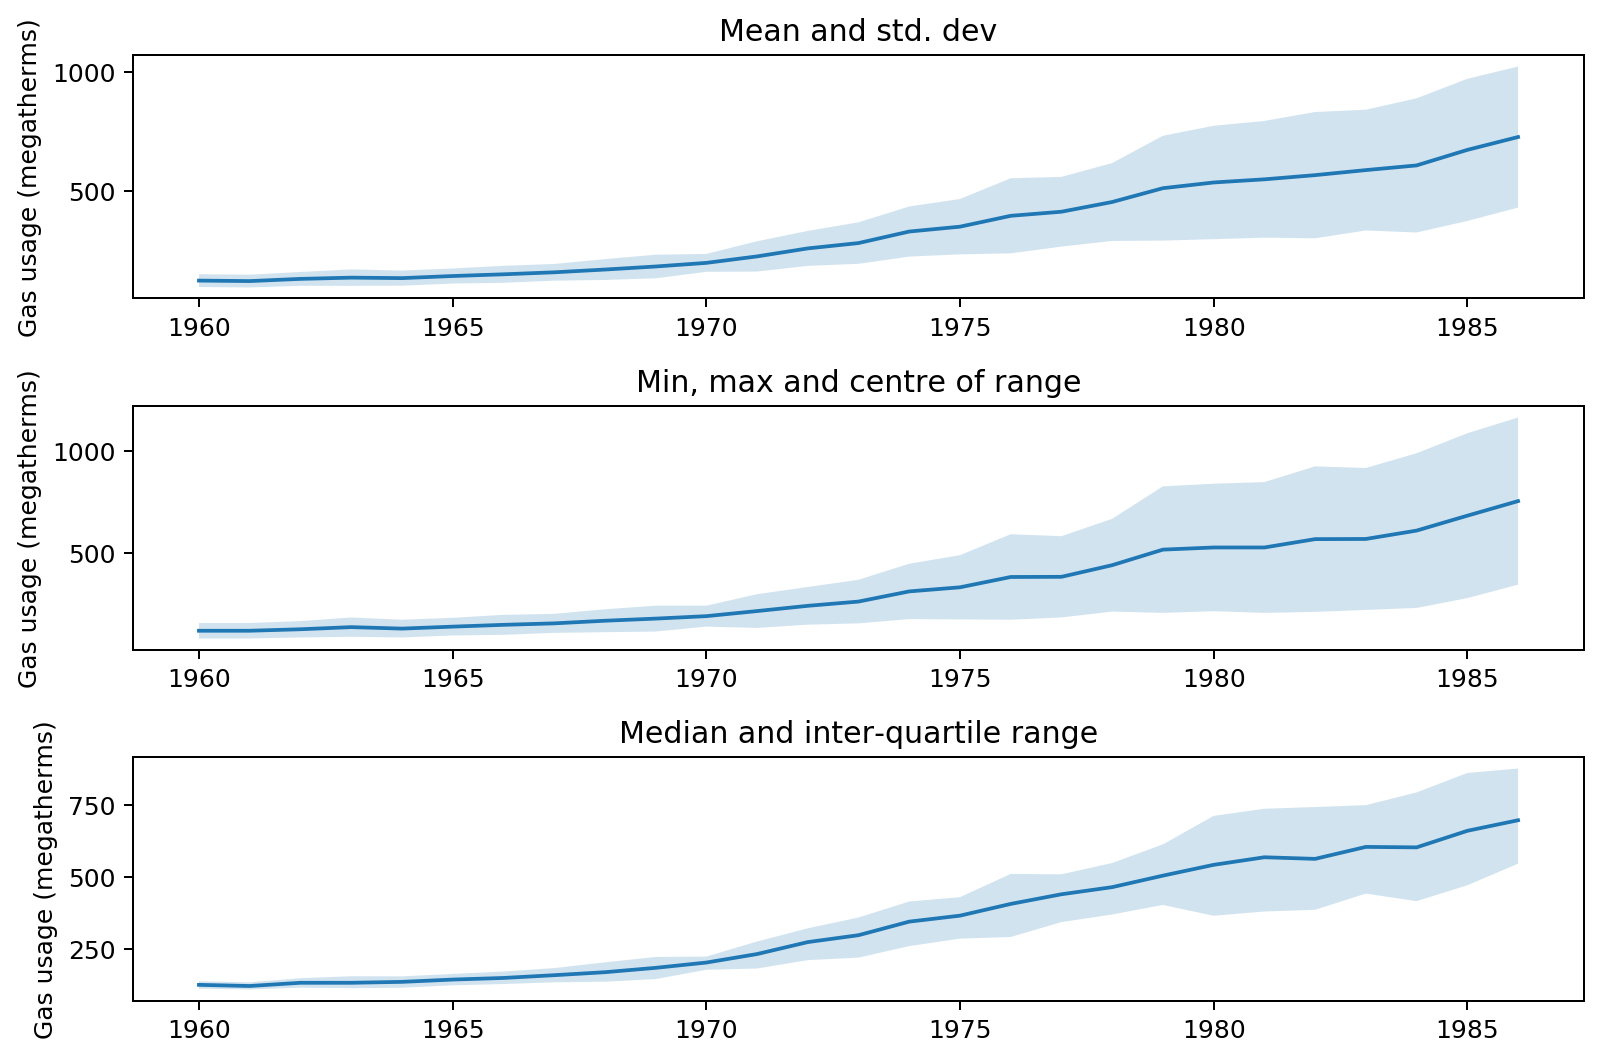
\includegraphics[scale=0.5]{src/2.32 Gas Example Plot 16.png}
    \caption{A faceted version of the gas example above, showing the mean, standard deviation, min, max and center of range, and median.}
\end{figure}
The 3 facets above show the labelled data. It is more common, however, to show all of this data in one geom- a box plot.

A box plot computes multiple stats of a dataset and combines them into one geom. It is great for seeing the distribution of the values in the dataset. Usually, the following are shown:
\begin{itemize}
    \item the interquartile range (the range between 25\% and 75\%)- this is shown as a box;
    \item the median- shown as a horizontal line;
    \item the extrema (often represents the 2.5\% and 98.5\% percentiles)- shown as whiskers; and
    \item the outliers (data outside the extrema)- shown as crosses/circles.
\end{itemize}
An example of a box plot is given below.
\begin{figure}[H]
    \centering
    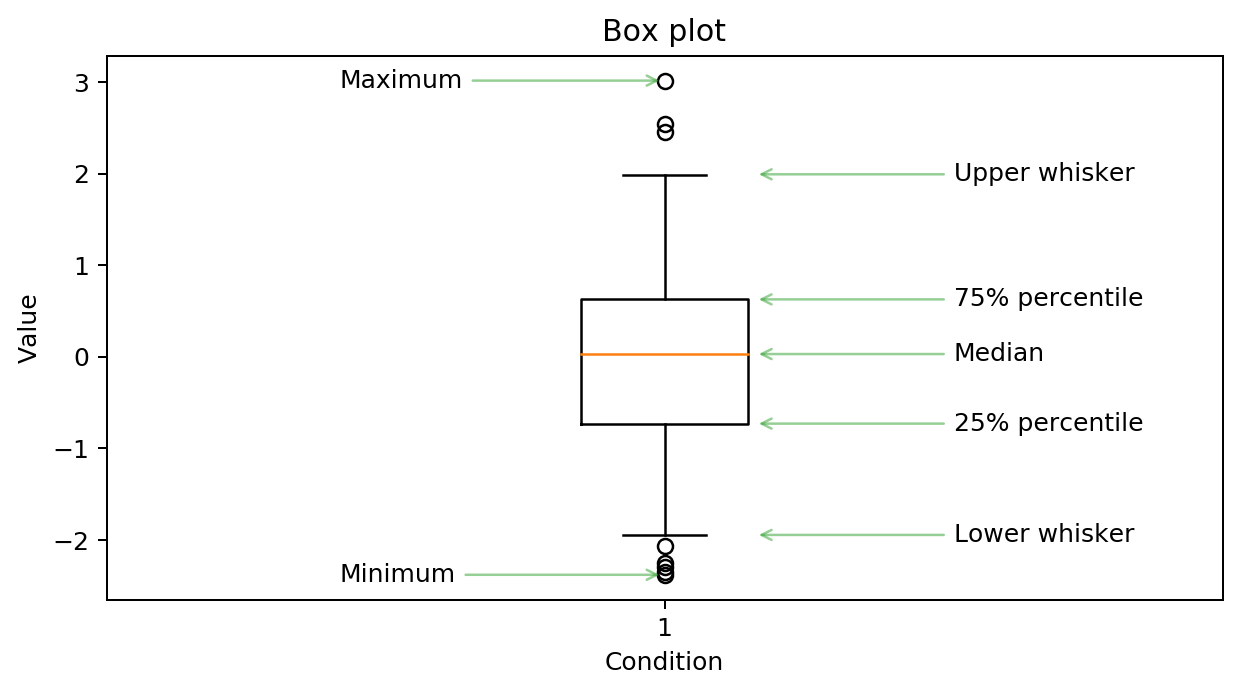
\includegraphics[scale=0.5]{src/2.33 Gas Example Plot 17.png}
    \caption{An example of a box plot.}
\end{figure}
\noindent Normally, they are used to plot different conditions and compare them.
\begin{figure}[H]
    \centering
    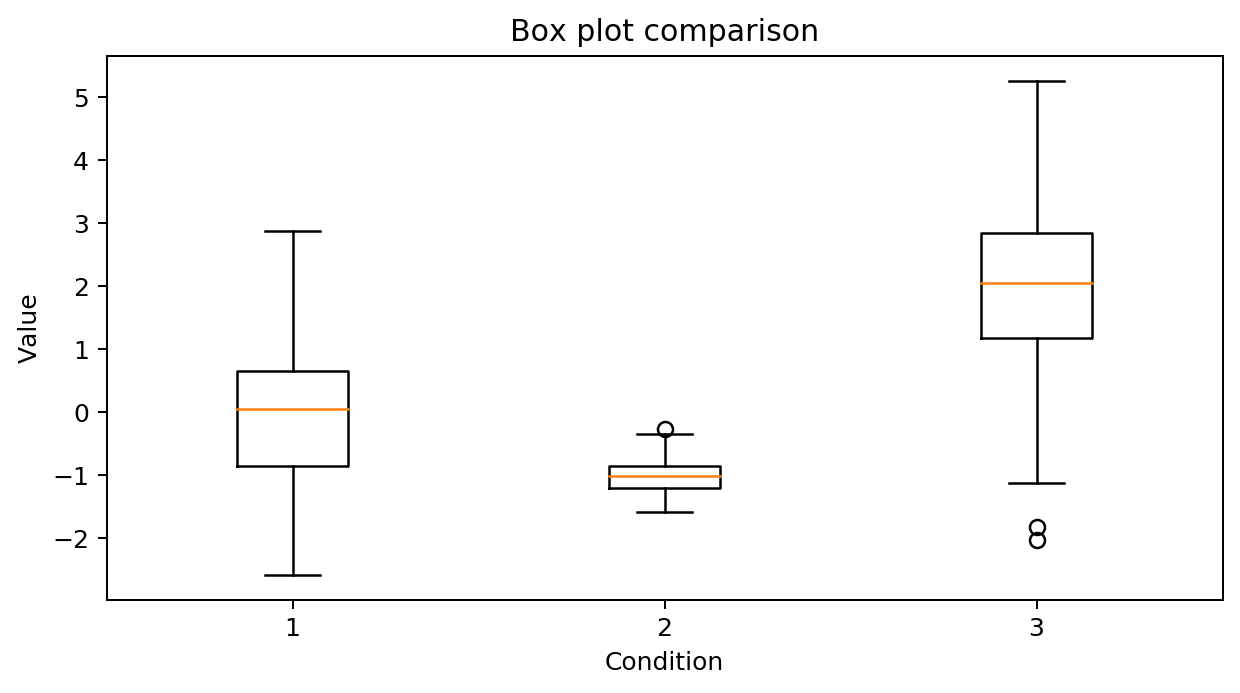
\includegraphics[scale=0.5]{src/2.34 Gas Example Plot 18.png}
    \caption{Using a box plot to show different conditions.}
\end{figure}

Instead of using box plots, we can use violin plots to represent the data more precisely. It plots the full distribution of the data, instead of a simple box. It uses the smoothing technique called kernel density estimate.
\begin{figure}[H]
    \centering
    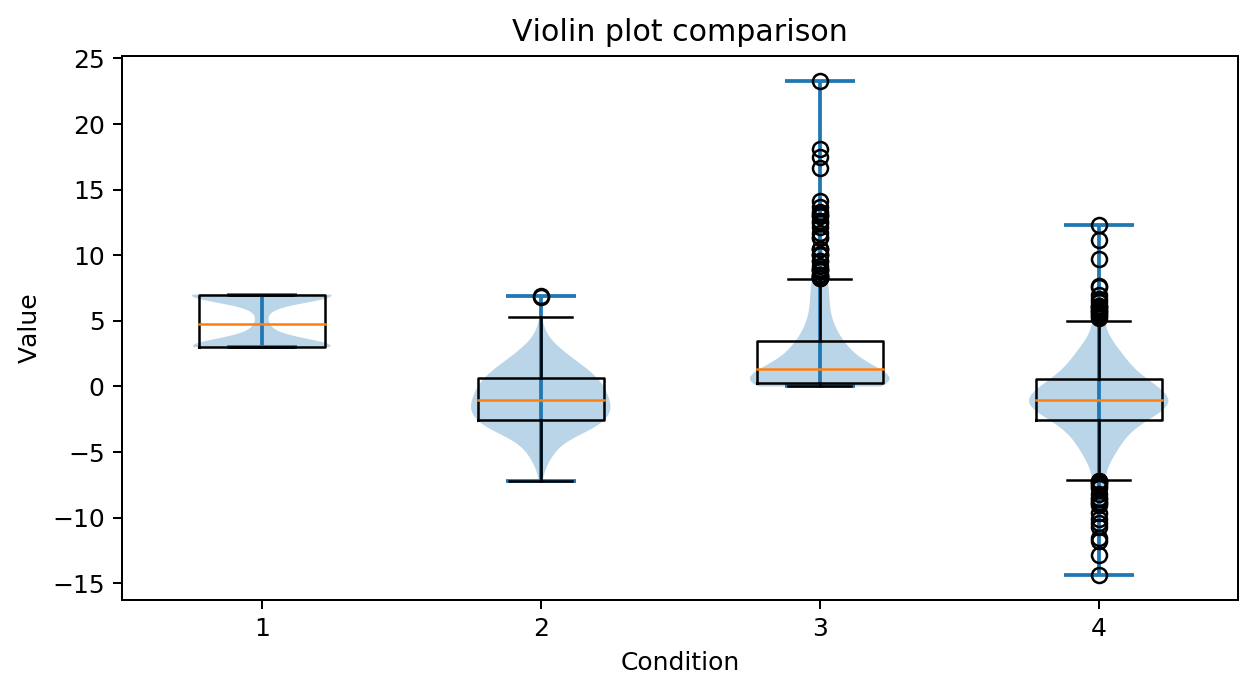
\includegraphics[scale=0.5]{src/2.35 Gas Example Plot 19.png}
    \caption{An example of a violin plot.}
\end{figure}

\subsection{Regression and Smoothing}
Regression finds an approximate function that closely matches the data. This function is usually simple. The most common type of regression is linear regression, i.e. fitting a line through the data. These are an important class of stats for proposing hypotheses to explain the pattern we see in data.
\begin{figure}[H]
    \centering
    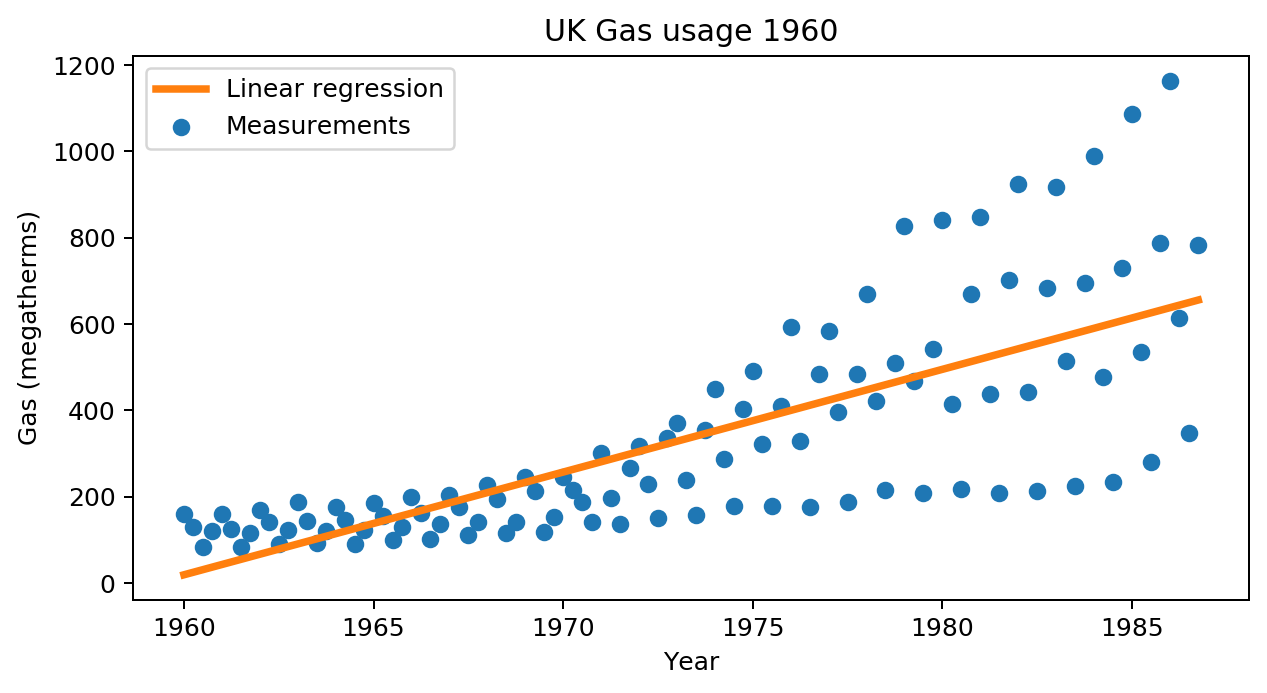
\includegraphics[scale=0.5]{src/2.36 Gas Example Plot 20.png}
    \caption{An example of a linear regression. The actual observations are shown as blue dots.}
\end{figure}
Instead of having a single line, we can have a moving average- it finds a simpler version of the data that hides changes within the dataset. This is smoothening of the data. A good smoothening reveals the important properties, while hiding the irrelevant ones.
\begin{figure}[H]
    \centering
    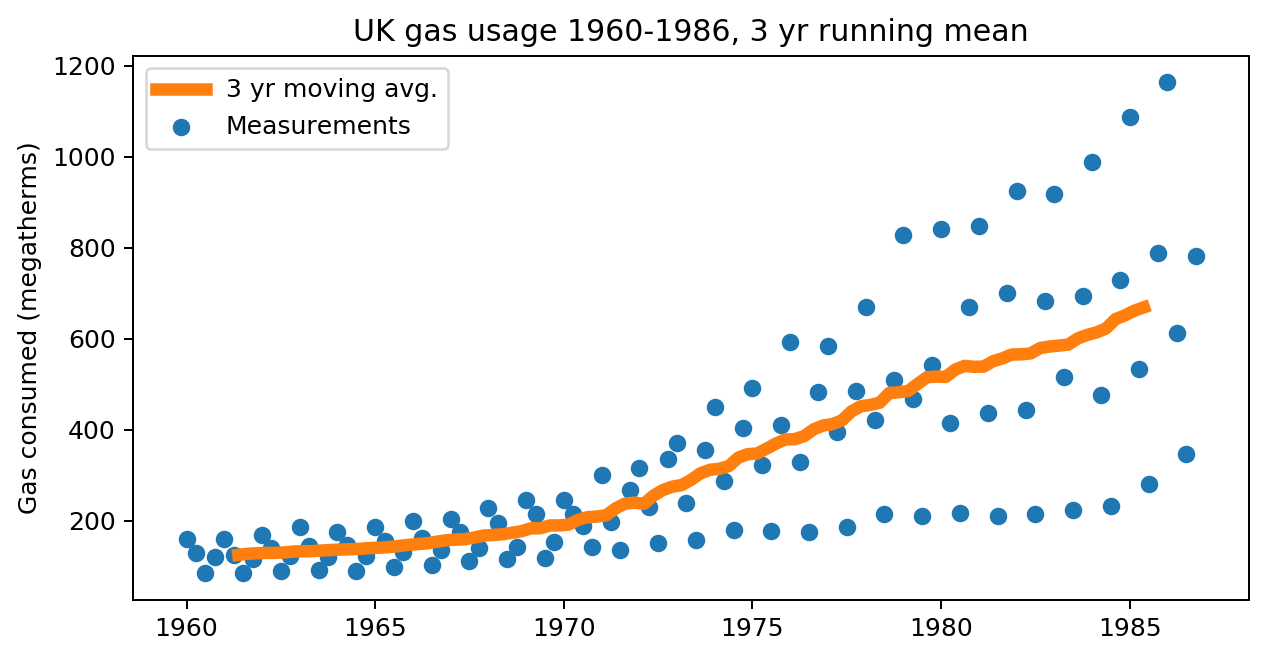
\includegraphics[scale=0.5]{src/2.37 Gas Example Plot 21.png}
    \caption{An example of a smoothenening of the line- this uses a 3 year running average.}
\end{figure}
\newpage

\section{Geoms and colour scales}
\subsection{Markers}
Markers are geoms that represent points in a coordinate system. These typically represent the raw data. They can just be points on the graph, but we can vary them to convey more information.

We can use different markers (i.e. different geoms) to distinguish different layers on the coordinate system. We can vary the shape and the colour of a marker.
\begin{figure}[H]
    \centering
    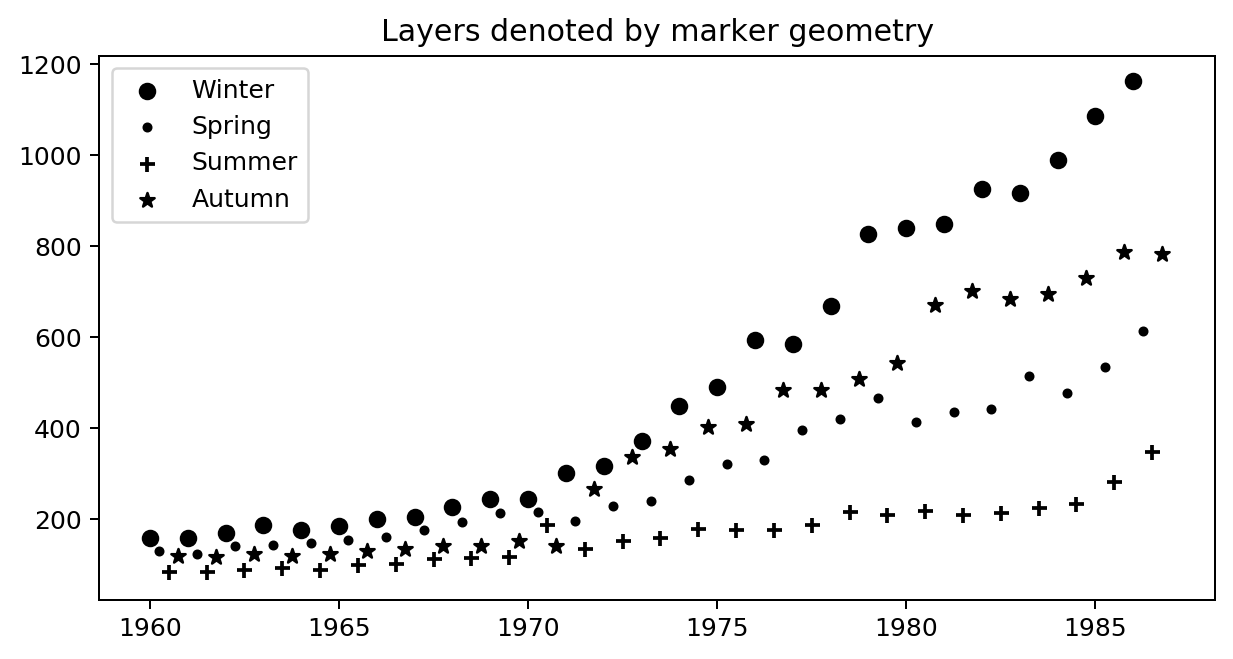
\includegraphics[scale=0.6]{src/2.38 Gas Example Plot 22.png}
    \caption{An example of graphs where the layers are distinguished by marker geometry.}
\end{figure}
\begin{figure}[H]
    \centering
    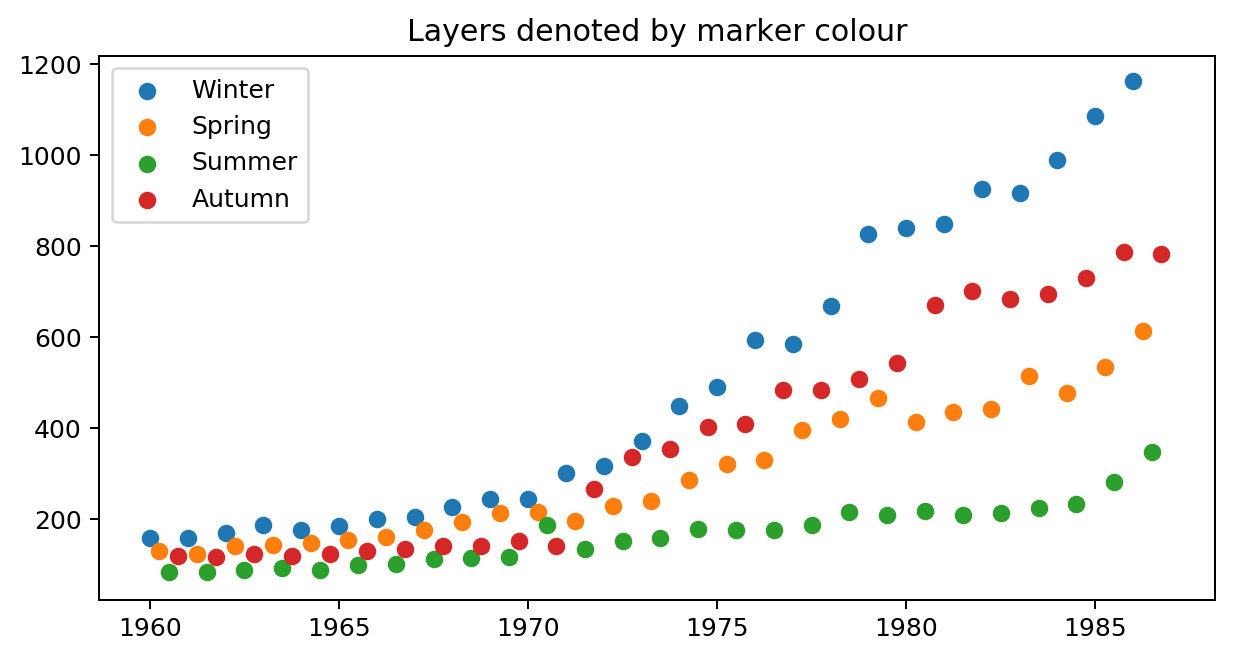
\includegraphics[scale=0.6]{src/2.39 Gas Example Plot 23.png}
    \caption{An example of graphs where the layers are distinguished by marker colour.}
\end{figure}
It is important to choose colours wisely. It is possible that the data might get printed in black and white. Moreover, a significant proportion of people people suffer some form of colour blindness, so we should avoid just separating layers using colour.

Instead of identifying layers, we can use markers to display another attribute. For example, we can vary the colour and the scale of the marker to convey some extra information. To see this, consider the following graph that shows earthquakes in Fiji.
\begin{figure}[H]
    \centering
    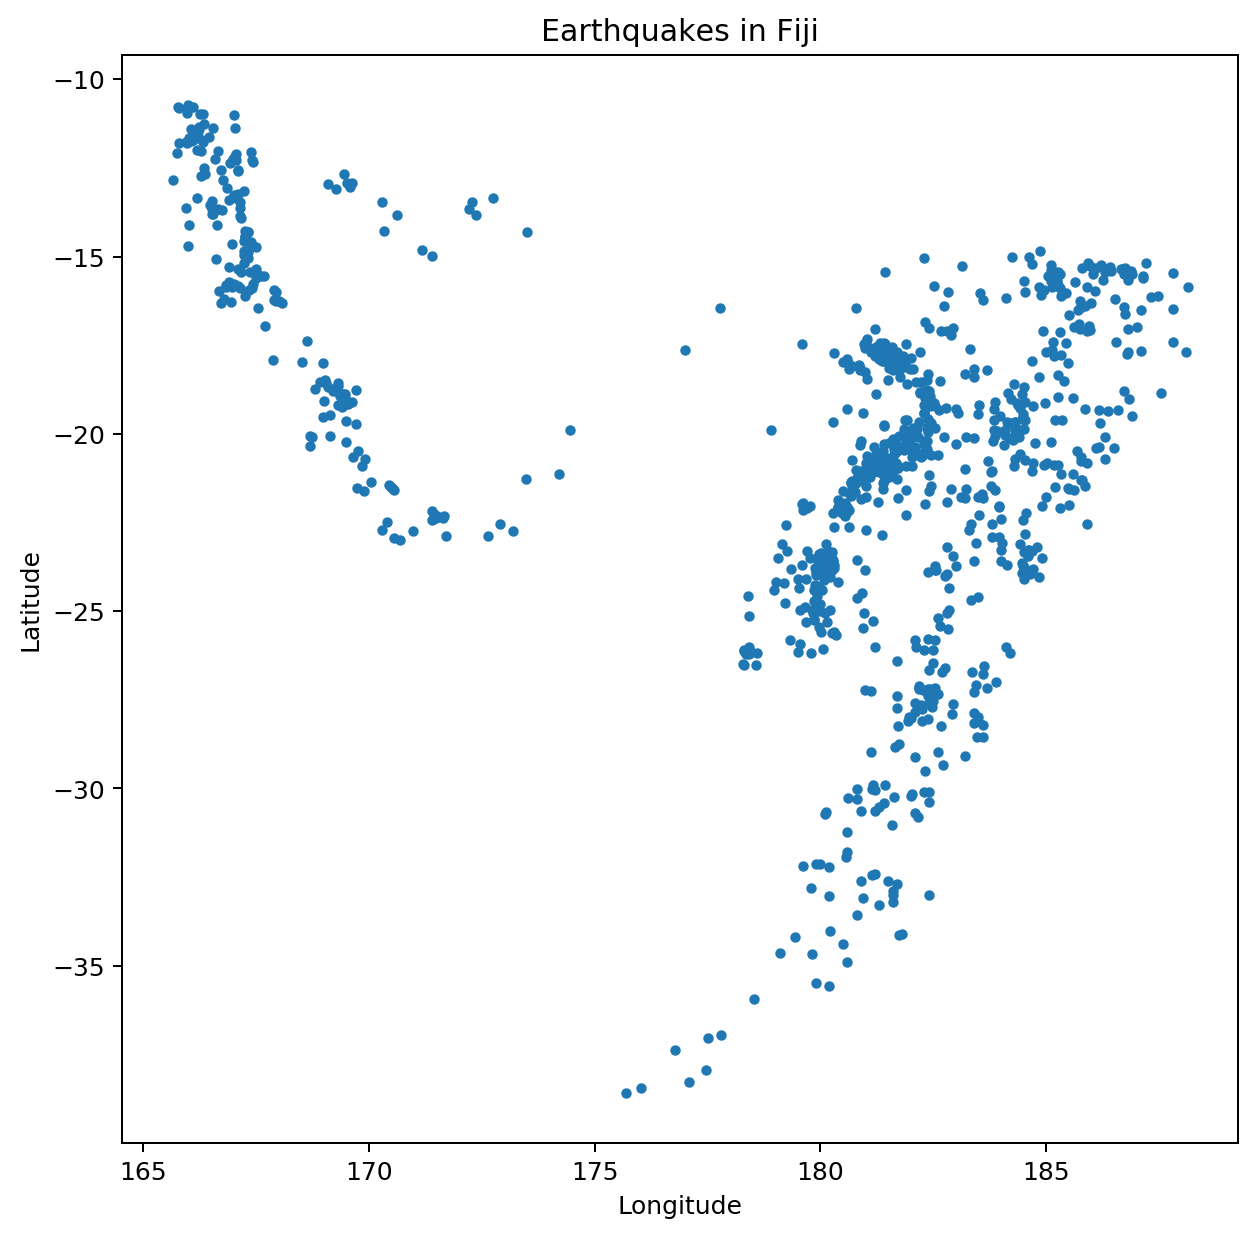
\includegraphics[scale=0.4]{src/2.40 Fiji Example Plot 1.png}
    \caption{A plot showing Earthquakes in Fiji, with respect to the latitutde and the longitude. The markers specify the location of the Earthquake.}
\end{figure}
\noindent We can use the size of the marker to display the magnitude of the earthquake.
\begin{figure}[H]
    \centering
    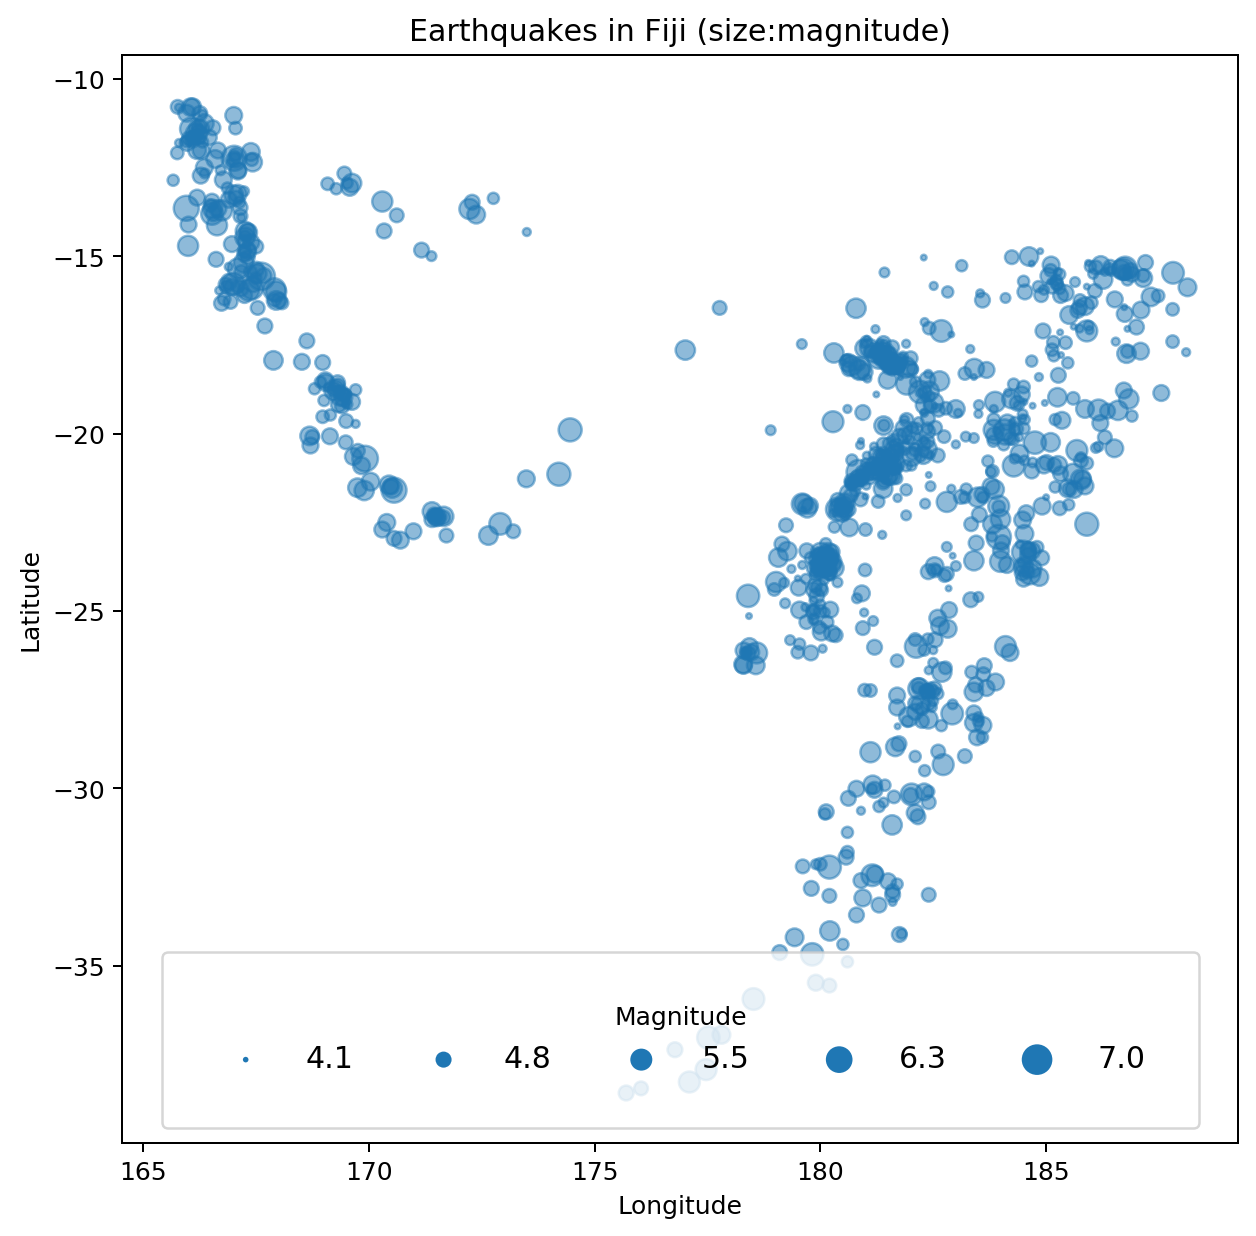
\includegraphics[scale=0.4]{src/2.41 Fiji Example Plot 2.png}
    \caption{A plot showing Earthquakes in Fiji, with respect to the latitutde and the longitude. The markers the location and the magnitude of the earthquake.}
\end{figure}
In the plot above, we have 3 variables- the longitude, latitutde and the magnitude of the earthquake. We can use colour to represent a further variable- depth of the earthquake.
\begin{figure}[H]
    \centering
    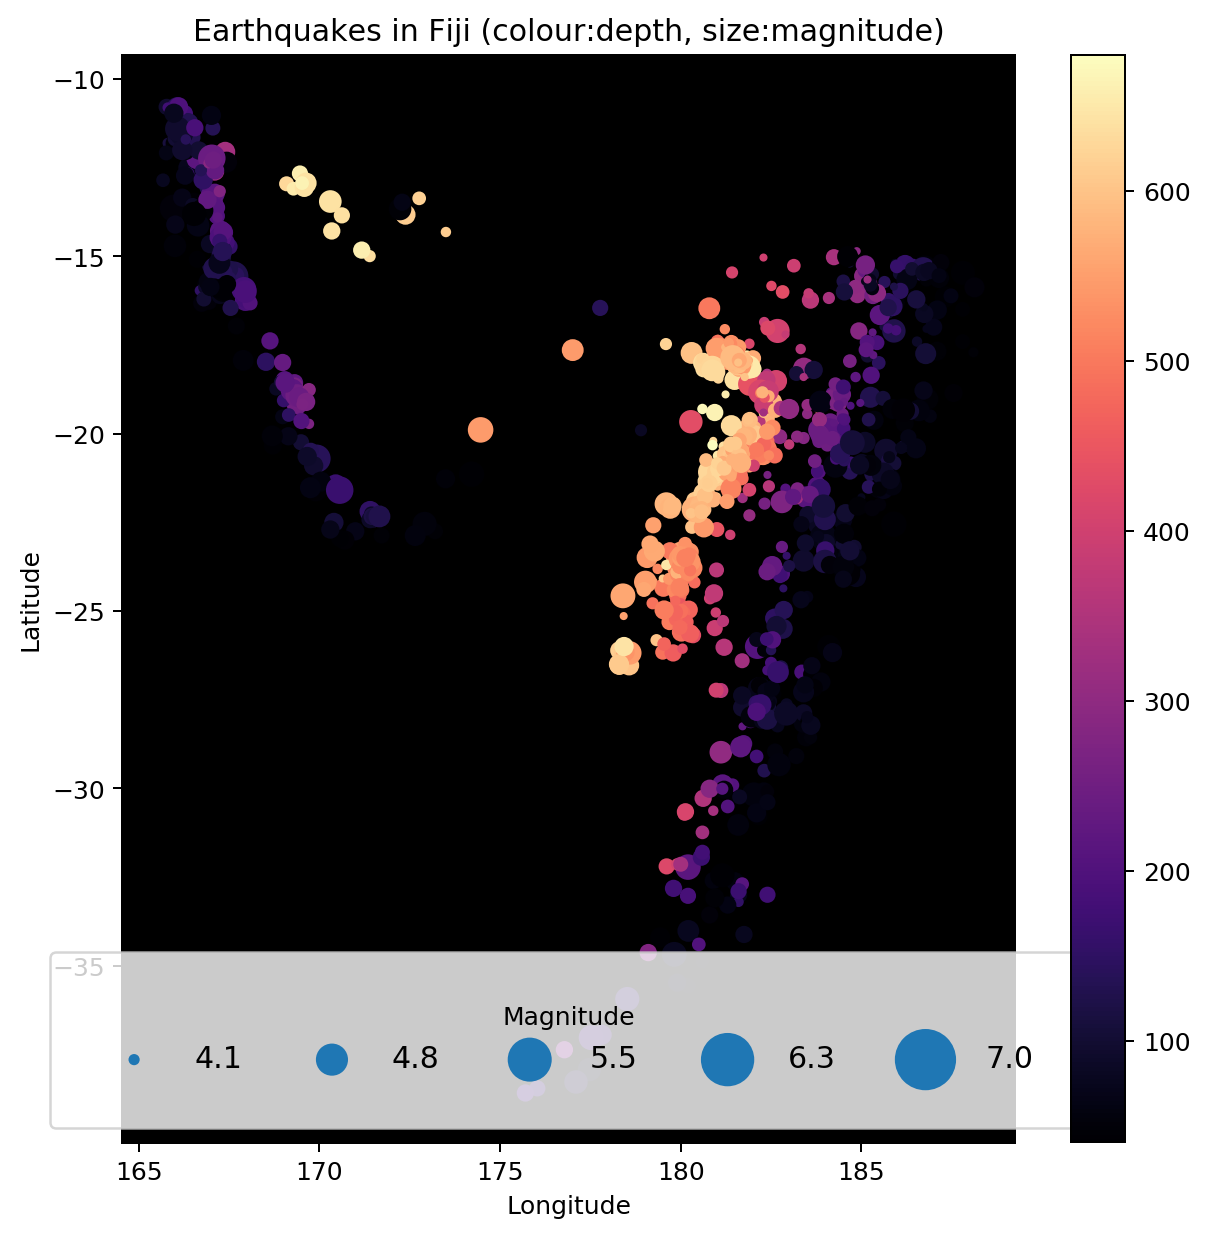
\includegraphics[scale=0.45]{src/2.42 Fiji Example Plot 3.png}
    \caption{A plot showing Earthquakes in Fiji, with respect to the latitutde and the longitude. The markers the location and the magnitude of the earthquake by size, and the depth of the earthquake by colour.}
\end{figure}

Colouring markers is done using a colour map- it maps scalars to colours. We should present a colour bar label along with the data- this is a guide, used for aesthetic mapping beyond the 2-variable plot.

While there are many colour maps possible, there are only few good choices. In general, there are 2 versions- one for unsigned/continuous values, and one for distinct values.

If the data is composed of positive scalars (e.g. heights of individuals), then we should use a colour map that varies monotonically with respect to brightness. That is, as the attribute increases, the colour gets lighter/darker consistently. In \texttt{matplotlib}, \texttt{vidris} and \texttt{magma} are good options for this. They are perceptually uniform, i.e. a change in value corresponds to a perceptually uniform change in colour intensity across the whole scale. It is possible to use grayscale/monchrome colour maps, but colours with brightness/hue are easier to interpret. As the data value increases, the visual brightness should also increase. A constant interval increase in data should lead to a perceptually constant increase in colour intensity.

Below, we have a colour mapping from \texttt{vidris} and \texttt{jet}.
\begin{figure}[H]
    \centering
    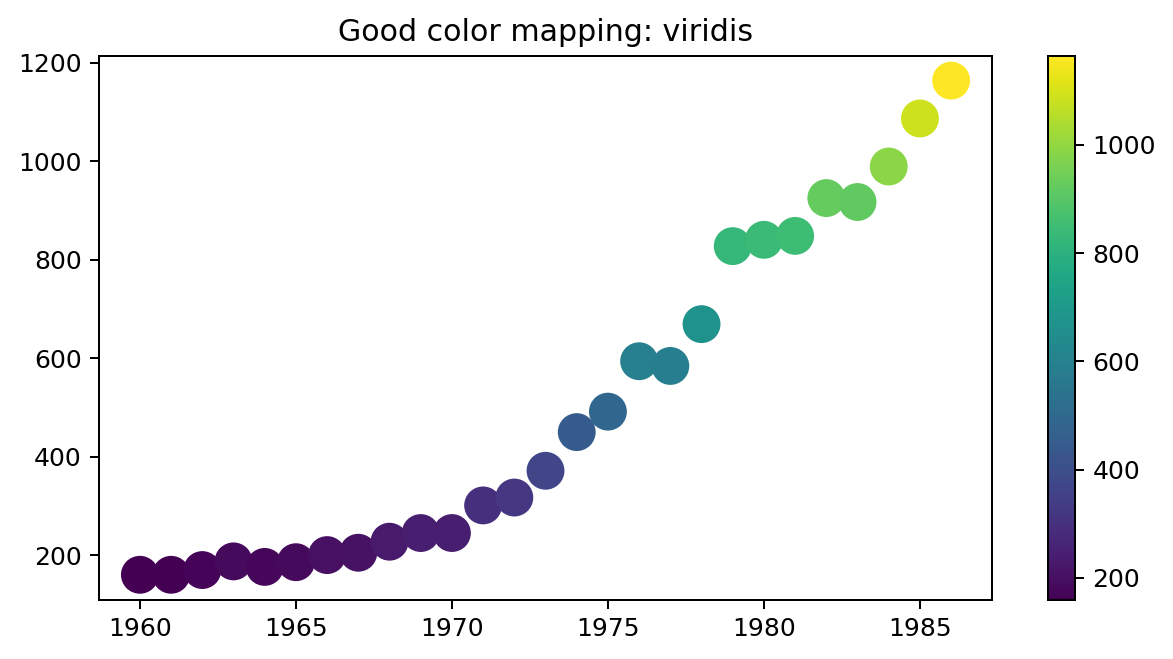
\includegraphics[scale=0.5]{src/2.43 vidris colour map.png}
    \caption{The vidris colour map.}
\end{figure}
\begin{figure}[H]
    \centering
    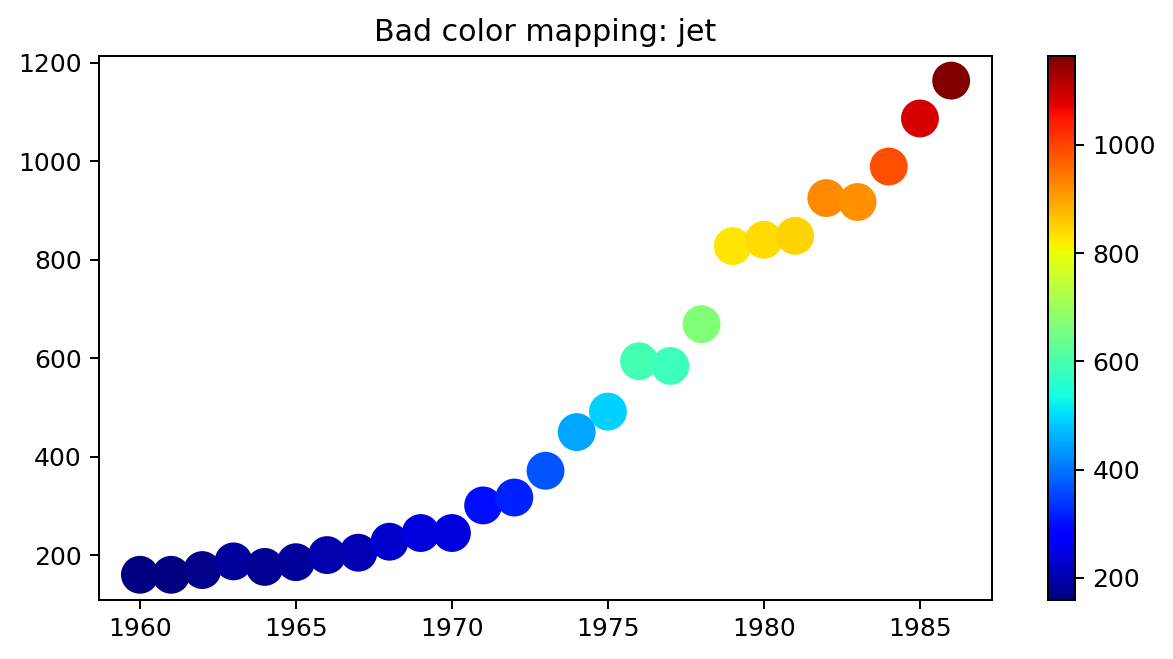
\includegraphics[scale=0.5]{src/2.44 jet colour map.png}
    \caption{The jet colour map.}
\end{figure}
\noindent The reason \texttt{jet} is bad is that it introduces false contours in visualisations- the markers do not have monotonic brightness.

If the data is signed (i.e. positive and negative), then the colour map should diverge around 0, and be monotonic in brightness around 0. A good example is given below.
\begin{figure}[H]
    \centering
    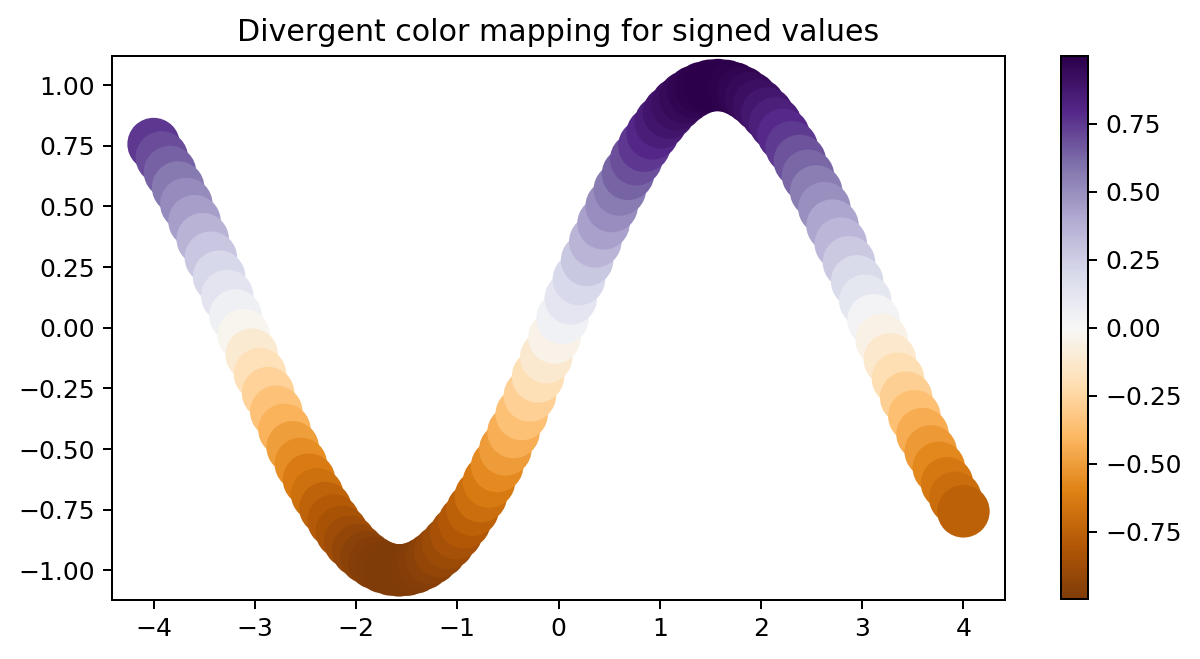
\includegraphics[scale=0.5]{src/2.45 Divergent colour mappings for signed values.png}
    \caption{Divergent colour mapping for signed values.}
\end{figure}
\noindent The following is a bad colour map since it does not converge at 0.
\begin{figure}[H]
    \centering
    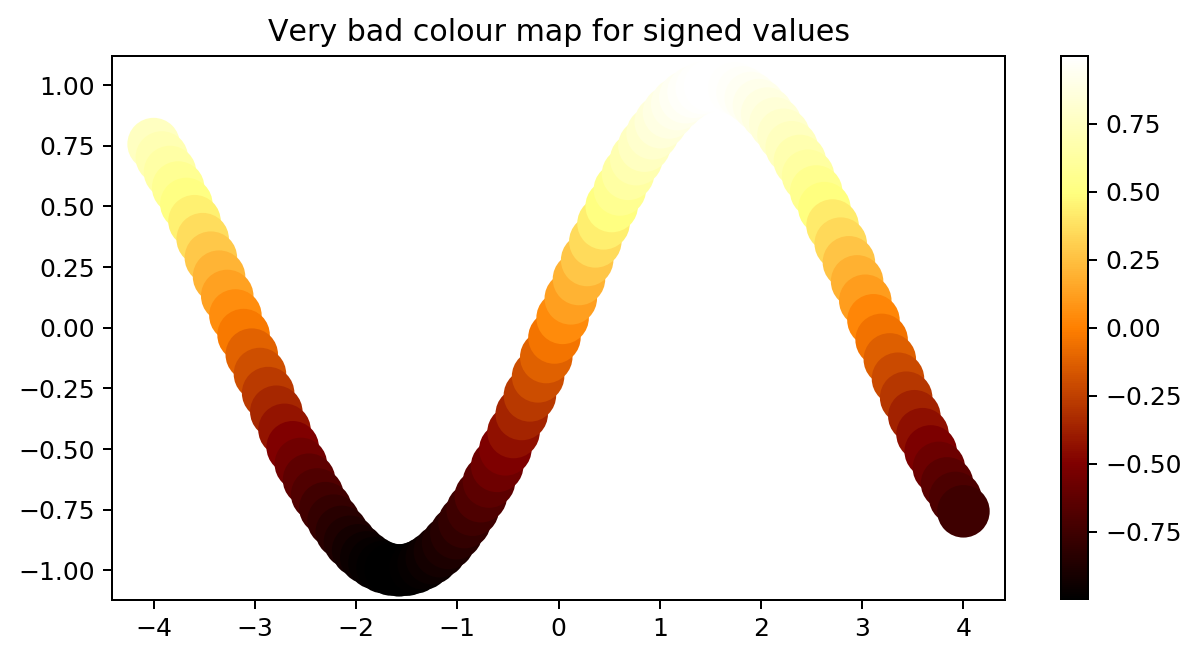
\includegraphics[scale=0.5]{src/2.46 Very bad colour map for signed values.png}
    \caption{Very bad colour map for signed values.}
\end{figure}
\noindent It should be possible to go back from the colour to the value using the label- the colour map guide is essential for this.

\subsection{Lines}
Lines are geoms that connect points in the dataset/stat. A line only makes sense if data can exist between two datapoints, i.e. there is a continuum of values. It is a good choice when we have two arrays which represent samples from an apparent continuous function. Line geoms can have variable thickness and colour, as shown in the example below.
\begin{figure}[H]
    \centering
    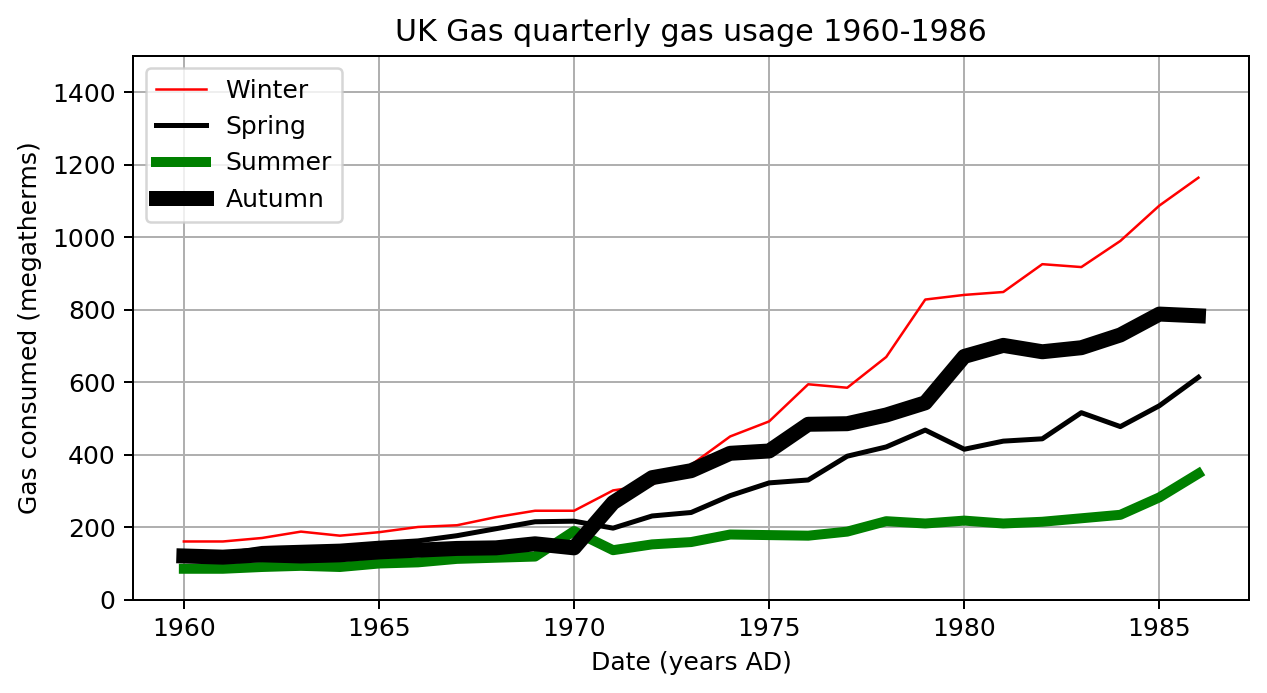
\includegraphics[scale=0.5]{src/2.47 linestyles.png}
    \caption{Data from the gas example split into quarters, with each line having variable line thickness and colour.}
\end{figure}
\noindent We can also vary dash patterns. This might be combined with colour changes to help those with colour blindness to interpret the figure. Nonetheless, it is a bad idea to use more than 4 dash patterns.
\begin{figure}[H]
    \centering
    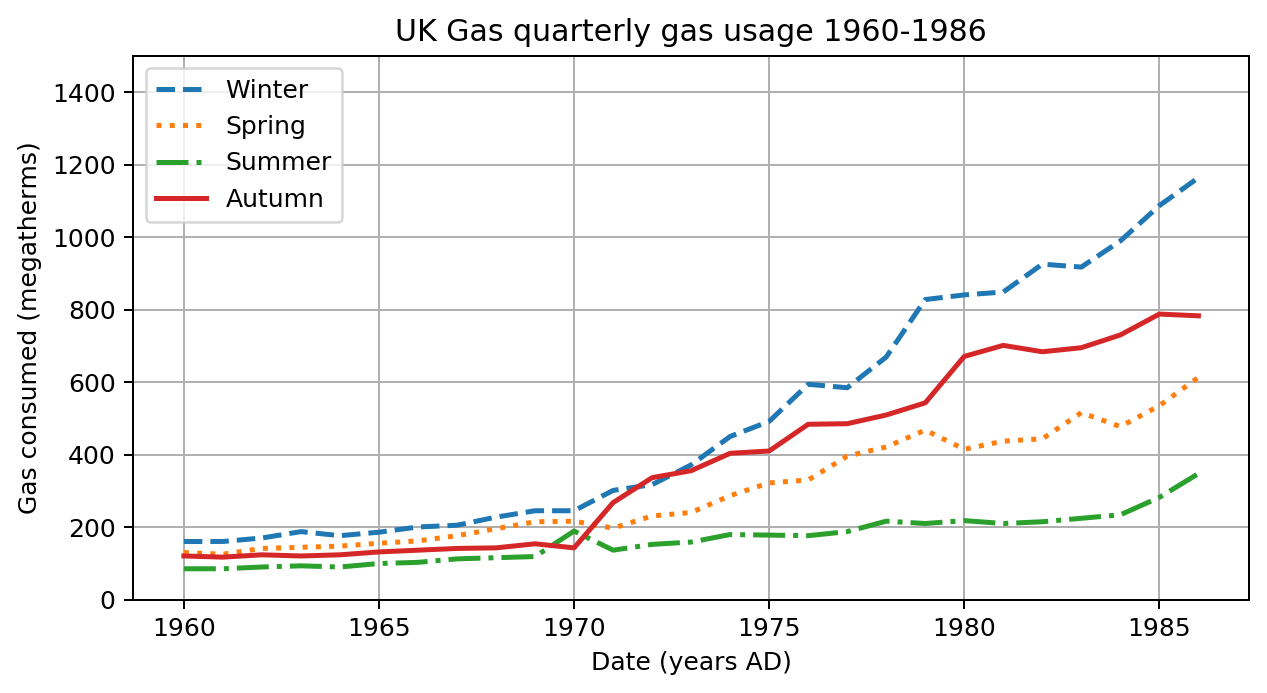
\includegraphics[scale=0.5]{src/2.48 dotstyle.png}
    \caption{Data from the gas example split into quarters, with each line having variable dash pattern.}
\end{figure}

If the data doesn't make sense as a line graph (e.g. half coin-tosses), then we can use the staircase approach to represent the data.
\begin{figure}[H]
    \centering
    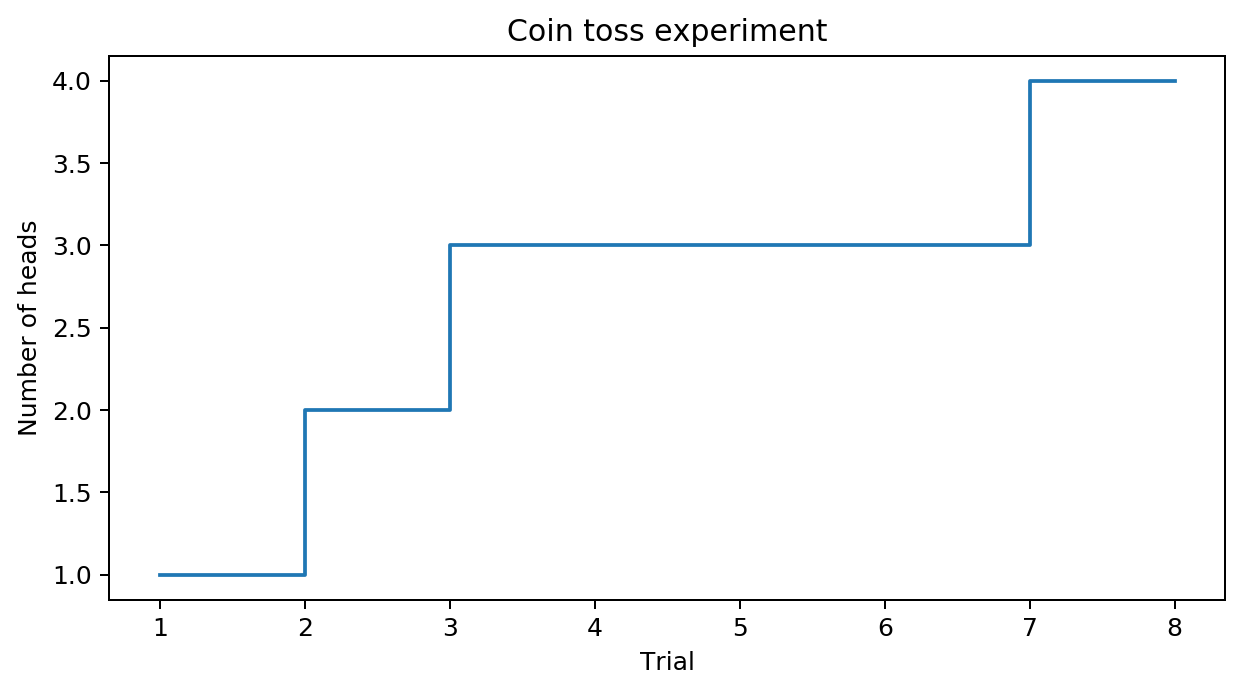
\includegraphics[scale=0.45]{src/2.49 coin toss jump.png}
    \caption{A coin toss experiment}
\end{figure}
\noindent As we can see above, the value here remains constant until the next observation, when it jumps to that position. There is no linear interpolation in the middle.

If the measurements of $x$ are discrete (e.g. conditions in an experiment), we should use a bar chart instead of a line chart.
\begin{figure}[H]
    \centering
    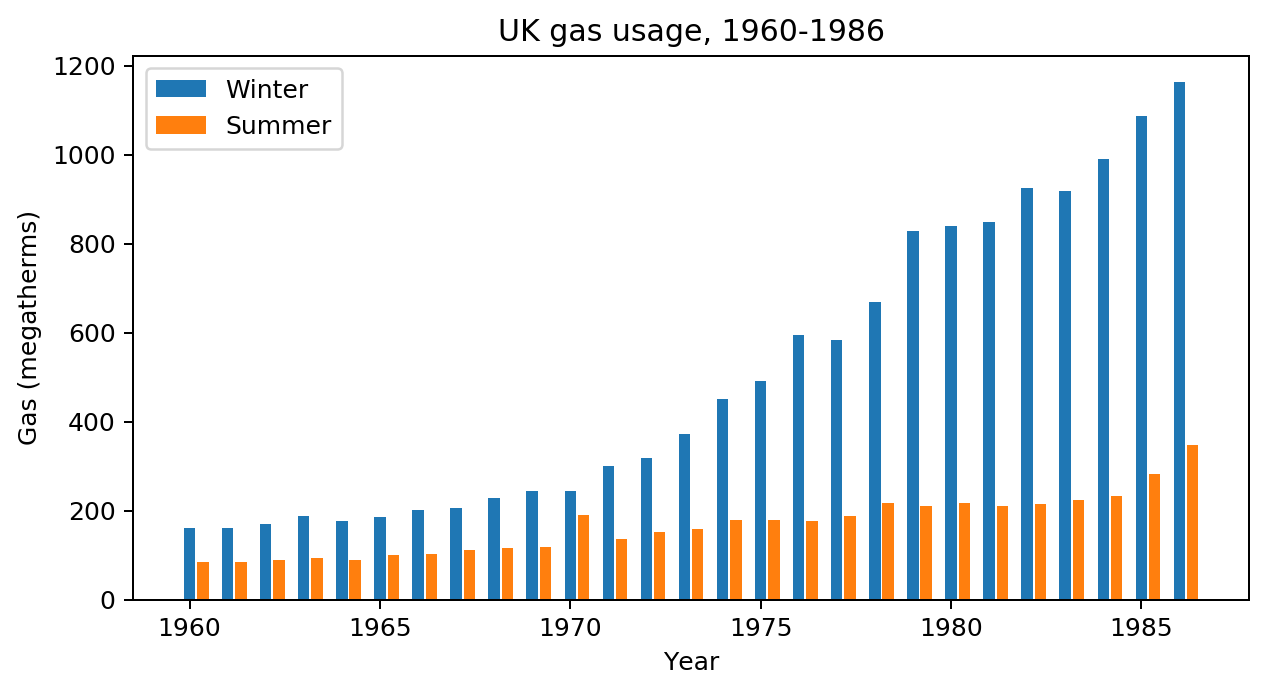
\includegraphics[scale=0.45]{src/2.50 bar chart.png}
    \caption{A bar chart}
\end{figure}

\subsection{Alphas and transparency}
We can render geoms with transparency, so that values behind can show clearly. This is called opacity (the inverse of transparency) or alpha. They can be used when large number of geoms overlap (e.g. on a dense scatterplot), or to (de)emphasise some geoms, along with line thickness. We should not use transparency a lot since it can make the data hard to see. Nonetheless, it can allow us to focus on certain geoms.
\begin{figure}[H]
    \centering
    \includegraphics[scale=0.6]{src/2.51 Fiji Example Plot 4.png}
    \caption{Earthquakes in Fiji without alpha}
\end{figure}
\begin{figure}[H]
    \centering
    \includegraphics[scale=0.6]{src/2.52 Fiji example Plot 5.png}
    \caption{Earthquakes in Fiji 5\% opacity}
\end{figure}
\newpage

\section{Coords}
We can specify visual units to present data with different shape. 
\begin{figure}[H]
    \centering
    \includegraphics[scale=0.6]{src/2.53 compact line graph.png}
    \caption{Compact line graph}
\end{figure}
\begin{figure}[H]
    \centering
    \includegraphics[scale=0.6]{src/2.54 wide line graph.png}
    \caption{Wide line graph}
\end{figure}
\noindent Similarly, we can use axis limits to specify the data unit range which is mapped on. 
\begin{figure}[H]
    \centering
    \includegraphics[scale=0.6]{src/2.55 axis limits.png}
    \caption{A line graph with different axis limits.}    
\end{figure}
\noindent Also, we can change the aspect ratio of the coordinate system. This can be used to ensure that images do not get stretched out/squashed.
\begin{figure}[H]
    \centering
    \includegraphics[scale=0.4]{src/2.56 aspect circle.png}
    \caption{Circle with different aspect ratios.}    
\end{figure}

A coordinate system projects data onto the 2D plane. We have only looked at the Cartesian plane until now, but we can transform it into log/polar coordinates, as we see fit.

If the data has large spans of magnitude, we should plot it in log coordinates. Log coordinates can be used in $x$-axis, $y$-axis, or both. If we have log on $x$ or $y$-axis, it is called semilog $x$ or semilog $y$. If we use it in both axes, it is called log-log.
\begin{figure}[H]
    \centering
    \includegraphics[scale=0.5]{src/2.57 log scale.png}
    \caption{A Cartesian vs log plot}    
\end{figure}
\noindent A function of the form $f(x) = x^k$ looks linear in a log-log plot.
\begin{figure}[H]
    \centering
    \includegraphics[scale=0.5]{src/2.58 linear v log log.png}
    \caption{A Cartesian vs log-log plot}    
\end{figure}

We cannot use log plots in every case- logarithms are only defined for strictly positive numbers. So, we cannot plot signed data on a log scale (without shifting it to strictly positive values). There are modified versions of the log scale that ignore some area around 0, and plot \texttt{log(abs(x))*sign(x)}. This is called the symmetric logarithm, or symlog. The area around 0 that is cut out is plotted linear, which distorts the plot.

For angular measurements, we can use polar coordinates. These have axes- radius $r$ and angle $\theta$.
\newpage

\section{Facets and Layers}
Multiple geoms can be rendered in the same visualisation as either:
\begin{itemize}
    \item distinct layers on the same coordinate system, or
    \item distinct facets on separate coordinate systems (with separate scales and guides).
\end{itemize}
Layering is more appropriate when the geoms are closely related, and the data mapping are in the same units. We need a legend (a guide) to distinguish the two layers.

For example, we can plot the price of wheat and weekly wage in the same plot- they have the same units.
\begin{figure}[H]
    \centering
    \includegraphics[scale=0.5]{src/2.59 layered components.png}
    \caption{A plot with 2 layers}
\end{figure}
\noindent We should not plot the ratio of the price and the wage in the same plot. Instead, they should be plotted in two different facets.
\begin{figure}[H]
    \centering
    \includegraphics[scale=0.6]{src/2.61 wheat example II.png}
    \caption{A figure with 2 facets- the first with 2 layers, and the second with 1.}    
\end{figure}
We could also use double $y$-axes. Here, the $x$-mapping layer is common for all the dataset, but there are 2 $y$-mapping layers. We have two (slightly) different coordinate systems layered over each other. This should be avoided as it can be confusing to interpret.

Like above, it is much better to use different facets; separate coordinate systems for separate aspects of the datset. Facets need not share anything in common. Nonetheless, if they show the same attribute, then it is a good idea to use the same scale (if possible) to make comparisons easy between the coords.

There are many ways to lay out facets in a figure, e.g. $2 \times 2, 4 \times 1$, etc.
\newpage

\section{Communicating uncertainity}
A figure must communicate uncertainity correctly and not mislead the reader. It is common to have observation error, so the samples obtained may not represent the true values. For example, the reading on a thermometer is not the true temperature of the air.

There are other possible sources of error, e.g. rounding errors in numerical simulations, uncertainity uncertainity over the right choice/its parameters. We can use stats such as standard deviation and interquartile range to show summaries of a collection of data. For example, in the vitamin C example, we can consider averages over different doses.
\begin{figure}[H]
    \centering
    \includegraphics[scale=0.6]{src/2.63 tooth length example I.png}
    \caption{The mean tooth length increase under two different vitamin C administration regimes}
\end{figure}
\noindent Although the data above shows the mean, the raw data was a sample of measurements, so we should represent the variation of data, e.g. using error bars.
\begin{figure}[H]
    \centering
    \includegraphics[scale=0.6]{src/2.64 tooth length example II.png}
    \caption{The mean tooth length increase under two different vitamin C administration regimes, with error bars}
\end{figure}

There are many choices for error bars, e.g.
\begin{itemize}
    \item standard deviations,
    \item standard error,
    \item confidence interval (e.g. 95\%), and
    \item non-parametric intervals (e.g. interquartile ranges).
\end{itemize}
Box plots are a good way of visualising the spread of values in a compact form.

An alternative is to jitter the points on the $x$-axis slightly. This is called dot plot.
\begin{figure}[H]
    \centering
    \includegraphics[scale=0.6]{src/2.66 dot plot.png}
    \caption{A dot plot}
\end{figure}
\noindent It is a good idea to use this with large collections of data.



\end{document}
